% SIAM Article Template
\documentclass{siamart0516}
\usepackage{subfig}
\usepackage{forest}
\usepackage[section]{placeins}
\usepackage[export]{adjustbox}
\usepackage[title]{appendix}
\usepackage{amssymb}
\usepackage{multirow}

\newcommand{\lp}{\left(}
\newcommand{\rp}{\right)}

\newcommand{\R}{\mathbb{R}}
\newcommand{\N}{\mathbb{N}}
\newcommand{\Z}{\mathbb{Z}}
\newcommand{\Q}{\mathbb{Q}}
\newcommand{\C}{\mathbb{C}}
\newcommand\supp{\mathop{\rm supp}}
\newcommand{\ct}{\mathcal{T}}
\newcommand{\Tm}{\ensuremath{\nu_\text{merge}}}
\newcommand{\num}{\ensuremath{\nu_\text{merge}}}

%%


\newcommand{\prop}[2]{\textsf{#1}(#2)}
\newcommand{\pp}[2]{\frac{\partial #1}{\partial #2}}

\newcommand{\vect}[1]{\mathbf{#1}}
\newcommand{\plotwidth}{0.45}
\newcommand{\WRP}{\par\qquad\(\hookrightarrow\)\enspace}
\newcommand{\ARP}{\par\qquad\ \enspace}
\DeclareMathOperator*{\argmax}{arg\,max}  % in your preamble
\DeclareMathOperator*{\argmin}{arg\,min}  % in your preamble 
%%%%% custom commands for this paper
\newcommand{\nmax}{N}
\newcommand{\bigo}{\mathcal{O}}
\newcommand{\child}[1]{\textsf{child}$_{#1}$}
\newcommand{\weight}[1]{w\textsubscript{#1}}
%%%%%


% Information that is shared between the article and the supplement
% (title and author information, macros, packages, etc.) goes into
% ex_shared.tex. If there is no supplement, this file can be included
% directly.
% SIAM Shared Information Template
% This is information that is shared between the main document and any
% supplement. If no supplement is required, then this information can
% be included directly in the main document.


% Packages and macros go here
\usepackage{lipsum}
\usepackage{amsfonts}
\usepackage{graphicx}
\usepackage{epstopdf}
\usepackage{algorithmic}
\ifpdf
  \DeclareGraphicsExtensions{.eps,.pdf,.png,.jpg}
\else
  \DeclareGraphicsExtensions{.eps}
\fi

% Add a serial/Oxford comma by default.
\newcommand{\creflastconjunction}{, and~}

% Used for creating new theorem and remark environments
\newsiamremark{remark}{Remark}
\newsiamremark{hypothesis}{Hypothesis}
\crefname{hypothesis}{Hypothesis}{Hypotheses}
\newsiamthm{claim}{Claim}


%\newcommand{\TheTitle}{An adaptive partition of unity method for Chebyshev polynomial interpolation on Hypercubes} 
%\newcommand{\TheAuthors}{Kevin W. Aiton, Tobin A. Driscoll}


% Sets running headers as well as PDF title and authors
\headers{Adaptive partition of unity}{Kevin W. Aiton, Tobin A. Driscoll}

% Title. If the supplement option is on, then "Supplementary Material"
% is automatically inserted before the title.
\title{Preconditioned nonlinear iterations for overlapping Chebyshev discretizations with partition of unity \thanks{Submitted to the editors May 1, xxxx.
\funding{This research was supported by National Science Foundation grant DMS-1412085.}}}

% Authors: full names plus addresses.
\author{Kevin W. Aiton, Tobin A. Driscoll}

\usepackage{amsopn}
\DeclareMathOperator{\diag}{diag}


%%% Local Variables: 
%%% mode:latex
%%% TeX-master: "ex_article"
%%% End: 


% Optional PDF information
\ifpdf
\hypersetup{
  pdftitle={\TheTitle},
  pdfauthor={\TheAuthors}
}
\fi

% The next statement enables references to information in the
% supplement. See the xr-hyperref package for details.

\externaldocument{ex_supplement}

% FundRef data to be entered by SIAM
%<funding-group>
%<award-group>
%<funding-source>
%<named-content content-type="funder-name"> 
%</named-content> 
%<named-content content-type="funder-identifier"> 
%</named-content>
%</funding-source>
%<award-id> </award-id>
%</award-group>
%</funding-group>

\begin{document}

\maketitle

% REQUIRED
\begin{abstract}
We are doing adaptive multivariate approximations, and it works pretty well. This is a working abstract.

\end{abstract}

% REQUIRED
\begin{keywords}
  partition of unity, Chebyshev interpolation, Chebfun, overlapping domain decomposition
\end{keywords}

% REQUIRED
\begin{AMS}
  	65L11, 65D05, 65D25
\end{AMS}

\section{Introduction}
\label{sec:introduction}

A distinctive and powerful mode of scientific computation has emerged recently in which mathematical functions are represented by high-accuracy numerical analogs, which are then manipulated or analyzed numerically using a high-level toolset~\cite{Trefethen2015}. The most prominent example of this style of computing is the open-source Chebfun project~\cite{battles2004extension,Driscoll2014}. Chebfun, which is written in MATLAB, samples a given piecewise-smooth univariate function at scaled Chebyshev nodes and automatically determines a Chebyshev polynomial interpolant for the data, resulting in an approximation that is typically within a small multiple of double precision of the original function. This approximation can then be operated on and analyzed with algorithms that are fast in both the asymptotic and real-time senses. Notable operations include rootfinding, integration, optimization, solution of initial- and boundary-value problems, eigenvalues of differential and integral operators, and solution of time-dependent PDEs.

Townsend and Trefethen extended the 1D Chebfun algorithms to 2D functions over rectangles in Chebfun2~\cite{townsend2013extension,Townsend2014}, which uses low-rank approximations in an adaptive cross approximation. The construction and manipulation of 2D approximations is suitably fast for a wide range of smooth examples. Most recently, Hashemi and Trefethen created an extension of Chebfun called Chebfun3 for 3D approximations on hyperrectangles using low-rank ``slice--Tucker'' decompositions~\cite{Hashemi2017}. The range of functions that Chebfun3 can cope with in a reasonable interactive computing time is somewhat narrower than for Chebfun2, as one would expect.

A distinctive aspect of the low-rank approximations used by Chebfun2 and Chebfun3 is that they are highly nonisotropic. That is, rotation of the coordinate axes can transform a rank-one or low-rank function to one with a much higher rank, greatly increasing the time required for function construction and manipulations. 

An alternative to Chebfun and related projects ported to other languages is sparse grid interpolation. Here one uses linear or polynomial interpolants on hierarchical Smolyak grids. Notable examples of software based on this technique are the Sparse Grid Interpolation Toolbox~\cite{Klimke2005} and the Sparse Grids Matlab Kit~\cite{Back2011}. An advantage of these packages is that they are capable of at least medium-dimensional representations on hyperrectangles. However, they are less fully featured than the Chebfun family. These methods are also highly nonisotropic.

In this work we propose decomposing a hyperrectangular domain by adaptive, recursive bisections in one dimension at a time, generalizing earlier work in one dimension\cite{Aiton2018}. The resulting subdomains are defined to be overlapping, and on each we employ simple tensor-product Chebyshev polynomial interpolants. In order to define a global smooth approximation, we use a partition of unity to blend together the subdomains. This allows the approximation to capture highly localized function features while remaining computationally tractable.

The more general problem of approximation of a function with high pointwise accuracy over a nonrectangular domain $\Omega \subset \R^d$ allows more limited global options than in the hyperrectangular case. Neither low-rank nor sparse grid approximations have any clear global generalizations to this case. Two techniques that can achieve spectral convergence for at least some such domains are radial basis functions~\cite{} and Fourier extension or continuation~\cite{adcock2014resolution}, but neither has been conclusively demonstrated to operate with high speed and reliability over a large collection of domains and functions.

Our use of an adaptive decomposition allows us to approximate on such domains with great flexibility. If a base subdomain is hyperrectangular, we proceed with a tensor-product interpolation for speed, but if its intersection with the global domain is nonrectangular, we can opt for a different representation. We need not be concerned with having a very large number of degrees of freedom in any local subproblem, since further subdivision is available, so the local algorithm need not be overly sophisticated. 


The adaptive construction of function approximations is based on binary trees, as explained in section~\ref{sec:construction}. In section~\ref{sec:operations} we describe fast algorithms for evaluation, arithmetic combination, differentiation, and integration of the resulting tree-based approximations. Numerical experiments in section~\ref{sec:numerical_experiments} demonstrate that the tree-based approximations exhibit far less anisotropy than do Chebfun2 and Chebfun3. Our implementation is faster than Chebfun2 and Chebfun3 on all tested examples---sometimes by orders of magnitude---except for examples of very low rank, for which all the methods are acceptably fast. In section~\ref{sec:general-domain} we describe and demonstrate approximation on nonrectangular domains using a simple linear least-squares approximation by the tensor-product Chebyshev basis. While these results are preliminary, we think they show enough promise to merit further investigation. 



\section{Adaptive construction}
\label{sec:construction}

Let $\Omega = \{ \vect{x} \in \R^d: x_i \in [a_i,b_i], i=1,\ldots,d\}$ be a hyperrectangle, and suppose we wish to approximate $f:\Omega \to \R$. Our strategy is to cover $\Omega$ with overlapping subdomains, on each of which $f$ is well-approximated by a multivariate polynomial, and use a partition of unity to construct a global approximation. We defer a description of the partition of unity scheme to section~\ref{sec:operations}. In this section we describe an adaptive procedure for obtaining the overlapping domains. 

The domains are constructed from recursive bisections of $\Omega$ into nonoverlapping hyperrectangular \emph{zones}. Let $t>0$ be a parameter. Given a zone $\prod_{j=1}^d [\alpha_{j},\beta_{j}]$, we extend it to a larger domain $\prod_{j=1}^d [\bar{\alpha}_{j},\bar{\beta}_{j}]$ by fixing a parameter $t>0$, defining
\begin{equation}
  \label{eq:overlap}
  \delta_{j} =  \frac{\beta_{j}-\alpha_{j}}{2}(1+t),\quad j=1,\ldots,d,
\end{equation}
and then setting
\begin{equation}
  \bar{\alpha}_{j} = \max\{a_j,\beta_{j}-\delta_{j}\}, \quad \bar{\beta}_{j} = \min\{\alpha_{j}+\delta_{j},b_j\}.
  \label{eq:zone_extend}
\end{equation}
In words, the zone is extended on all sides by an amount proportional to its width in each dimension, up to the boundary of the global domain $\Omega$. 


We define a binary tree $\ct$ with each node $\nu$ having the following properties:
\begin{itemize}
\item \prop{zone}{$\nu$}: zone associated with $\nu$
\item \textsf{domain}($\nu$): domain associated with $\nu$
\item \textsf{isdone}($\nu$): $n$-vector of boolean values, where $\textsf{isdone}_j$ indicates whether the domain is determined to be sufficiently resolved in the $j$th dimension
\item \child{0}($\nu$),\child{1}($\nu$): left and right subtrees of $\nu$ (empty for a leaf)
\item \textsf{splitdim}($\nu$): the dimension in which $\nu$ is split (empty for a leaf)
\end{itemize}

\noindent A leaf node has the following additional properties:
\begin{itemize}
\item \textsf{grid}($\nu$): tensor-product grid of Chebyshev 2nd-kind points mapped to \prop{domain}{$\nu$}
\item \textsf{values}($\nu$): function values at \textsf{grid}($\nu$)
\item \textsf{interpolant}($\nu$): polynomial interpolant of \textsf{values}($\nu$) on \textsf{grid}($\nu$)
\end{itemize}

\noindent If $\nu$ is a leaf, its domain is constructed by extending \prop{zone}{$\nu$} as in~(\ref{eq:zone_extend}). Otherwise, \prop{domain}{$\nu$} is the smallest hyperrectangle containing the domains of its children. 

Let $f$ be the scalar-valued function on $\Omega$ that we wish to approximate. A key task is to compute, for a given leaf node $\nu$, the polynomial \textsf{interpolant}($\nu$), and determine whether $f$ is sufficiently well approximated on \textsf{domain}($\nu$) by it. First we sample $f$ at a Chebyshev grid of size $\nmax^d$ on \textsf{domain}($\nu$). This leads to the interpolating polynomial
\begin{equation}
  \label{eq:full-interp}
  \tilde{p}(\vect{x}) = \sum_{i_1=0}^{\nmax-1} \cdots \sum_{i_d=0}^{\nmax-1}  C_{i_1,\ldots,i_d} T_{i_1}(x_1)\cdots T_{i_d}(x_d),
\end{equation}
where the coefficient array $C$ can be computed by an $n$-dimensional FFT in $\bigo(\nmax^d \log \nmax)$ time~\cite{mason2002chebyshev}. Following the practice of Chebfun3t \cite{Hashemi2017}, for each $j=1,\ldots,d$, we define a scalar sequence $\gamma^{(j)}$ by summing $|C_{i_1,\ldots,i_d}|$ over all dimensions except the $j$th. To each of these sequences we apply Chebfun's {\tt StandardChop}  algorithm, which attempts to measure decay in the coefficients in a suitably robust sense~\cite{Aurentz:2017:CCS:3034774.2998442}. Let the output of {\tt StandardChop} for sequence $\gamma^{(j)}$ be $n_j$; this is the degree that {\tt StandardChop} deems to be sufficient for resolution at a user-set tolerance.  If $n_j<\nmax$ we say that the function is resolved in dimension $j$ on $\nu$. If $f$ is resolved in all dimensions on $\nu$, then we truncate the interpolant sums in~(\ref{eq:full-interp}) at the degrees $n_j$ and store the samples of $f$ on the corresponding smaller tensor-product grid. 

\begin{algorithm}
\caption{refine($\nu$,$f$,$\nmax$,$t$)}
\label{alg:refine}
\begin{algorithmic}
  \IF{$\nu$ is a leaf}
    \STATE Sample $f$ on \textsf{grid}($\nu$)
    \STATE Determine chopping degrees $n_1,\ldots,n_d$
    \FOR{each $j$ with \textsf{isdone}($\nu$)$_j=$ FALSE}
      \IF{$n_j<\nmax$}
        \STATE \textsf{isdone}($\nu$)$_j$ := TRUE
      \ELSE
        \STATE split($\nu$,$j$,$t$)
      \ENDIF
    \ENDFOR
    \IF{all \textsf{isdone}($\nu$) are TRUE}
      \STATE Truncate~(\ref{eq:full-interp}) at degrees $n_1,\ldots,n_d$ to define \textsf{grid}($\nu$), \textsf{values}($\nu$), \textsf{interpolant}($\nu$)
    \ELSE
      \STATE refine($\nu$,$\nmax$,$t$)
    \ENDIF
  \ELSE
    \STATE refine(\child{0}($\nu$),$\nmax$,$t$)      
    \STATE refine(\child{1}($\nu$),$\nmax$,$t$)
  \ENDIF
\end{algorithmic}
\end{algorithm}

Algorithm~\ref{alg:refine}  describes a recursive adaptation procedure for building the binary tree $\ct$, beginning with a root node whose zone and domain are both the original hyperrectangle $\Omega$. For a non-leaf input, the algorithm is simply called recursively on the children. For an input node that is currently a leaf of the tree, the function $f$ is sampled, and chopping is used in each unfinished dimension to determine whether sufficient resolution has been achieved. Each dimension that is deemed to be resolved is marked as finished. If all dimensions are found to be finished, then the interpolant is chopped to the minimum necessary length in each dimension, and the node will remain a leaf. Otherwise, the node is split in all unfinished dimensions using Algorithm~\ref{alg:split}, and Algorithm~\ref{alg:refine} is applied recursively. Note that the descendants of the splitting(s) inherit the \textsf{isdone} property that marks which dimensions have been finished, so no future splits are possible in such dimensions within this branch. 

\begin{algorithm}
\caption{split($\nu$,$j$,$t$)}
\label{alg:split}
\begin{algorithmic}
\IF{$\nu$ is a leaf}
\STATE \textsf{splitdim}($\nu$)=$j$
\STATE Define new nodes $\nu_0$, $\nu_1$
\STATE $[a_1,b_1],[a_2,b_2],\dots,[a_n,b_n]$ be the subintervals from \prop{zone}{$\nu$}
\STATE Let $m:= \frac{b_j+a_j}{2}$
\STATE Let \textsf{zone}($\nu_0$) $:= [a_1,b_1] \times \dots \times [a_{j-1},b_{j-1}] \times [a_{j},m] \times [a_{j+1},b_{j+1}] \times \dots \times [a_{d},b_{d}] $
\STATE Let \textsf{zone}($\nu_1$) $:= [a_1,b_1] \times \dots \times [a_{j-1},b_{j-1}] \times [m,b_{j}] \times [a_{j+1},b_{j+1}] \times \dots \times [a_{d},b_{d}] $
\FOR{$k=0,1$}
\STATE Define \textsf{domain}($\nu_k$) from \textsf{zone}($\nu_k$) with parameter $t$ as in~(\ref{eq:zone_extend})
\STATE Define \textsf{grid}($\nu_k$) as Chebyshev tensor-product grid of size $\nmax^d$ in \textsf{domain}($\nu_k$)
\STATE Let \textsf{isdone}($\nu_k$):= \textsf{isdone}($\nu$)
\ENDFOR
\ELSE
\STATE split(\child{0}($\nu$),$k$,$t$)
\STATE split(\child{1}($\nu$),$k$,$t$)
\ENDIF
\end{algorithmic}
\end{algorithm}

% Given a tree node $\nu$, we define a procedure sample($\nu$,$f$) as follows. Let $X^1, \dots, X^n$ be Chebyshev grids of length $d_1, \dots, d_n$  mapped to the intervals $[\bar{a}_1,\bar{b}_1], \dots [\bar{a}_n,\bar{b}_n]$ that define \textsf{domain}($\nu$). 

%Chebfun includes a splitting algorithm to create piecewise polynomial approximations \cite{pachon2010piecewise}. Here, the tolerance {\tt chebfuneps} used in {\tt StandardChop} is set to 
%\begin{equation}\text{{\tt chebfuneps*max(vscaleGlobal/vscaleLocal,hscale)}}, 	
%\end{equation}
%where {\tt vscaleGlobal},{ \tt vscaleLocal} and {\tt hscale} are estimates of the scales of the global function, local function, and interval width respectively \cite{Aurentz:2017:CCS:3034774.2998442}. We utilize this by keeping track of the scales. For example suppose we are testing in the first dimension. In our method {\tt vscaleGlobal} is set to the global sampled absolute maximum sampled value over the whole tree (which is kept track of when sampling), {\tt vscaleLocal} to the maximum absolute value locally sampled, and {\tt hscale} is set to the length of the domain of the dimension we are testing in (i.e. {\tt hscale}=$b_1-a_1$ if testing along the $x$-direction).

 % If the function is determined to be fully resolved on node $\nu$ in a dimension $j$, then the $j$th element of the array unfinished($\nu$) is set to false. This property is inherited by all the descendants of $\nu$, on the assumption that dimension $j$ will remain resolved in all future splittings of $\nu$. We keep track of this with the unfinished($\nu$) array where we set $\text{unfinished($\nu$)}_k$ to FALSE if the interpolant for $\nu$ can be refined in dimension $k$. We set unfinished(root($T$)) to an array of all TRUE values, and when splitting a leaf $\nu$ passes unfinished($\nu$) to the children of $\nu$. 

%We choose to split in the dimension $j$ of greatest length of the cuboid, excluding dimensions that have been determined to be refined for itself or any of the leaf's ancestors in the tree. For a leaf $\nu$, we keep track of this with the unfinished($\nu$) array where we set $\text{unfinished($\nu$)}_k$ to FALSE if the interpolant for $\nu$ can be refined in dimension $k$. We set unfinished(root($T$)) to an array of all TRUE values, and when splitting a leaf $\nu$ passes unfinished($\nu$) to the children of $\nu$. Thus we split in the the dimension $j$ where
%\begin{equation}
%j = \underset{j}{\mathrm{argmax}}\{(b_j - a_j): \text{unfinished($\nu$)}_j=\text{TRUE}\},	
%\end{equation}
%as seen in Algorithm~\ref{alg2}.




% If there are one or more unfinished dimensions which are found to be unresolved, node $\nu$ is split in each unfinished dimension, where we first split the node in the first unfinished dimension, and recursively split the children of $\nu$ in the subsequent unfinished dimensions as seen in Algorithm~\ref{alg2}. When we split a leaf $\nu$ to \child{0}($\nu$) and \child{1}($\nu$), the zones of the children are formed by splitting the \zone{\nu} in half along a dimension by a hyperplane; this is demonstrated in Algorithm~\ref{alg9}. 


% This process is recursively  repeated on the leaves until every leaf is determined to be resolved in every dimension. When recursing, we redefine the domains of non-leaf nodes $\nu$ to be the smallest hypercuboid that contains the domains of \child{0}($\nu$) and \child{1}($\nu$). In Algorithm~\ref{alg2} we show formally how we split the leaves. The binary tree representing the approximation is formed with Algorithm~\ref{alg3}, where sample($\nu$,$f(\vect{x})$) samples $f(\vect{x})$ on the Chebyshev tensor product grids at the leaves of $\nu$.


\section{Computations with the tree representation}
\label{sec:operations}

The procedure of the preceding section constructs a binary tree $\ct$ whose leaves each hold an accurate representation of $f$ over a subdomain. These subdomains overlap, and constructing a global partition of unity approximation from them is straightforward.

Define the $C^\infty$ function
\begin{align}
  \label{eq:basic-cinf}
  \psi_0(x) = \begin{cases}
    \exp \lp  1 - \frac{1}{1-x^2}\rp & |x| \leq 1, \\
    0 & |x| > 1,
  \end{cases}
\end{align}
and let
\begin{equation}
  \label{eq:affine}
  \ell(x;a,b) = 2\frac{x-a}{b-a} - 1
\end{equation}
be the affine map from $[a,b]$ to $[-1,1]$. Suppose $\nu$ is a leaf of $T$ with domain $\Omega_\nu = \prod [\bar{\alpha}_j,\bar{\beta}_j]$. Then we can define the smoothed-indicator or bump function
\begin{equation}
  \label{eq:bump-functions}
  \psi_\nu(\vect{x}) = \prod_{j=1}^d \psi_0\bigl( \ell(x_j;\bar{\alpha}_{j},\bar{\beta}_{j}) \bigr).
\end{equation}
Next we use Shepard's method~\cite{wendland2004scattered} to define a partition of unity $\{w_\nu (\vect{x})\}$, indexed by the leaves of $T$:
\begin{equation}
  \label{eq:pu-weight}
  w_\nu(\vect{x}) = \frac{\psi_\nu(\vect{x})}{\displaystyle \sum_{\mu\in \text{leaves}(\ct)} \psi_\mu(\vect{x})}.
\end{equation}
Let $s_\nu$ be the polynomial interpolant of $f$ over the domain of node $\nu$. Then the global approximant is
\begin{equation}
  s(\vect{x}) = \sum_{\nu\in \text{leaves}(\ct)} w_\nu(\vect{x})s_\nu(\vect{x}).
  \label{eq:pu-approx}	
\end{equation}

Next we describe efficient algorithms using the tree representation of the global approximant to perform common numerical operations such as evaluation at points, basic binary arithmetic operations on functions, differentiation, and integration.

\subsection{Evaluation}

Note that (\ref{eq:pu-weight})--~(\ref{eq:pu-approx}) can be rearranged into
\begin{equation}
  s(\vect{x}) = \sum_{\nu\in \text{leaves}(\ct)} \frac{s_\nu(\vect{x}) \psi_\nu(\vect{x})}{\displaystyle \sum_{\mu\in \text{leaves}(\ct)} \psi_\mu(\vect{x})}
  = \frac{\displaystyle\sum_{\nu\in \text{leaves}(\ct)} s_\nu(\vect{x}) \psi_\nu(\vect{x})}{\displaystyle \sum_{\mu\in \text{leaves}(\ct)} \psi_\mu(\vect{x})}.
  \label{eq:pu-alt}
\end{equation}
This formula suggests a recursive approach to evaluating the numerator and denominator, presented in Algorithm~\ref{alg:numden}. Using it, only leaves containing $\vect{x}$ and their ancestors are ever visited. A similar approach was described in~\cite{tobor2006reconstructing}.

\begin{algorithm}
\caption{[$S$,$P$]=numden($\nu$,$\vect{x}$)}
\label{alg:numden}
\begin{algorithmic}
\STATE $S=0$, $P=0$
\IF{$\nu$ is a leaf}
\STATE $S=\psi_\nu(\vect{x})$
\STATE $P = S \cdot \text{interpolant}(\nu)(\vect{x})$
\ELSE
\FOR{$k=0,1$}
\IF{$\vect{x} \in \text{\textsf{domain}(\child{k}}(\nu))$}
\STATE $[S_k,P_k]$ = numden(\child{k}($\nu$),$\vect{x}$) 
\STATE $S = S + S_k$
\STATE $P = P + P_k$
\ENDIF
\ENDFOR
\ENDIF
\end{algorithmic}
\end{algorithm}

Algorithm~\ref{alg:numden} can easily be vectorized to evaluate $s(\vect{x})$ at multiple points, by recursively calling each leaf with all values of $\vect{x}$ that lie within its domain. In the particular case when the evaluation is to be done at all points in a Cartesian grid, it is worth noting that the leaf-level interpolant in~(\ref{eq:full-interp}) can be evaluated by a process that yields significant speedup over a naive approach. As a notationally streamlined example, say that the desired values of $\vect{x}$ are $(\xi_{j_1},\ldots,\xi_{j_d})$, where each $j_k$ is drawn from $\{1,\ldots,M\}$, and that the array of polynomial coefficients is of full size $O(N^d)$. Express~(\ref{eq:full-interp}) as
\begin{multline}
  \label{eq:grid-eval}
  \sum_{i_1=0}^{\nmax-1} \cdots \sum_{i_d=0}^{\nmax-1}  C_{i_1,\ldots,i_d} T_{i_1}(\xi_{j_1})\cdots T_{i_d}(\xi_{j_d})
  \\ = \sum_{i_1=0}^{\nmax-1} T_{i_1}(\xi_{j_1}) \sum_{i_2=0}^{\nmax-1} T_{i_2}(\xi_{j_2}) \cdots \sum_{i_d=0}^{\nmax-1}  C_{i_1,\ldots,i_d} T_{i_d}(\xi_{j_d}).
\end{multline}
The innermost sum yields $N^{d-1}M$ unique values, each taking $\bigo(N)$ time to compute. At the next level there are $N^{d-2}M^2$ values, and so on, finally leading to the computation of all $M^d$ interpolant values. This takes $\bigo(MN(M+N)^{d-1})$ operations, as opposed to $\bigo(M^dN^d)$ when done naively. 



\subsection{Binary arithmetic operations}

Suppose we have two approximations $\hat{s}_1(\vect{x})$, $\hat{s}_2(\vect{x})$, represented by trees $\ct_1$ and $\ct_2$ respectively, and we want to construct a tree approximation for $\hat{s}_1 \circ \hat{s}_2$, where $\circ$ is one of the operators $+$, $-$, $\times$, or $\div$. If $\ct_1$ and $\ct_2$ have identical tree structures, then it is straightforward to operate leafwise on the polynomial approximations. In the cases of multiplication and division, the resulting tree have to be refined further using Algorithm~\ref{alg:split}, since these operations typically result in polynomials of degree greater than the operands. 

If the trees $\ct_1$ and $\ct_2$ are not structurally identical, we are free to use Algorithm~\ref{alg:split} to construct an approximation by sampling values of $\hat{s}_1 \circ \hat{s}_2$. However, the tree of $\hat{s}_1 \circ \hat{s}_2$ likely shares refinement structure with both $ct_1$ and $ct_2$. For example, Figure~\ref{zone_tan} shows the refined zones of the trees for $\arctan(100(x^2+y))$, $\arctan(100(x+y^2))$, and their sum. Thus in practice we merge the trees $\ct_1$ and $\ct_2$ using Algorithm~\ref{alg:merge}, presented in Appendix~\ref{sec:merge}. The merged tree, whose leaves contain sampled values of the result, may then be refined further if chopping tests then reveal that the result is not fully resolved. 

\begin{figure}
\centering
\subfloat[Zone plot of $f_1(x,y)$]{
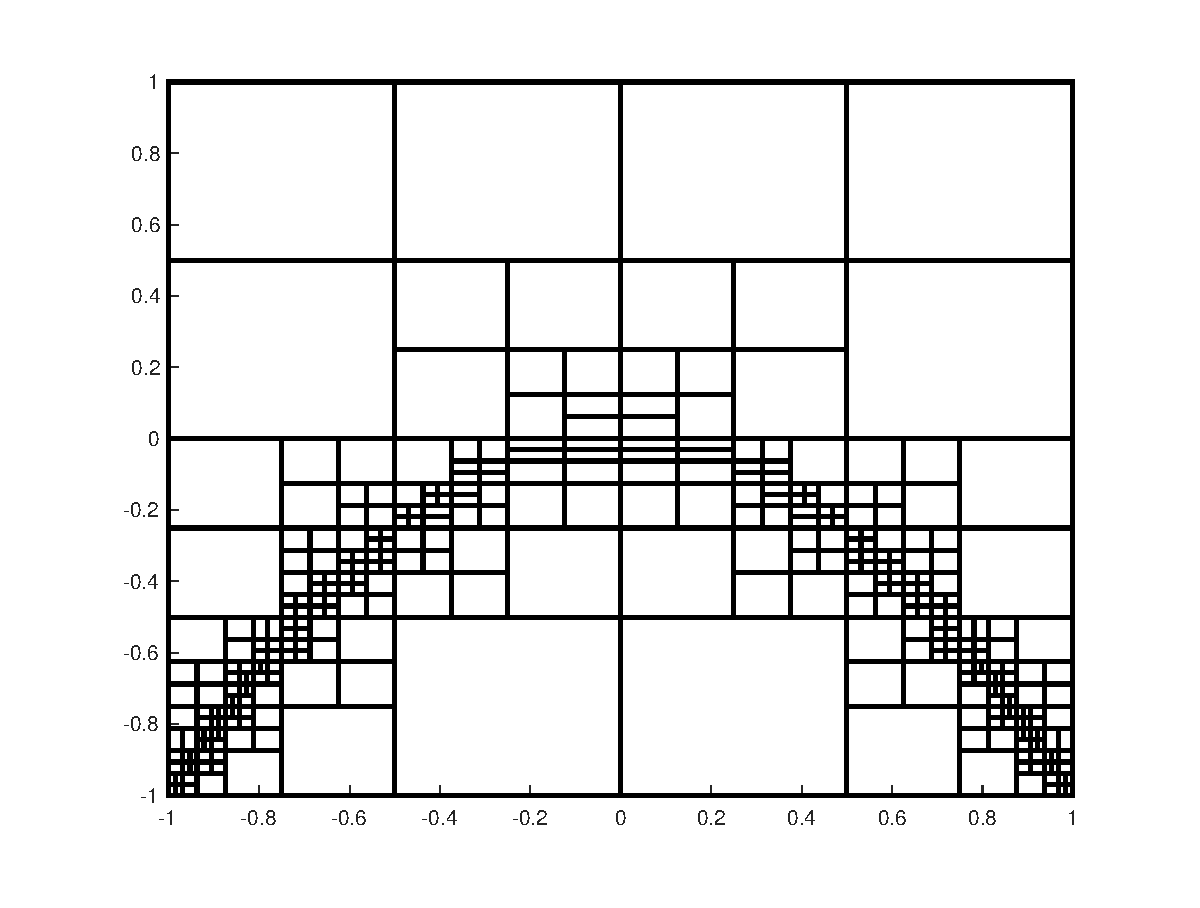
\includegraphics[scale = 0.3]{tan_100_1.eps}
   \label{zone_tan_a}
 }
\subfloat[Zone plot of $f_2(x,y)$]{
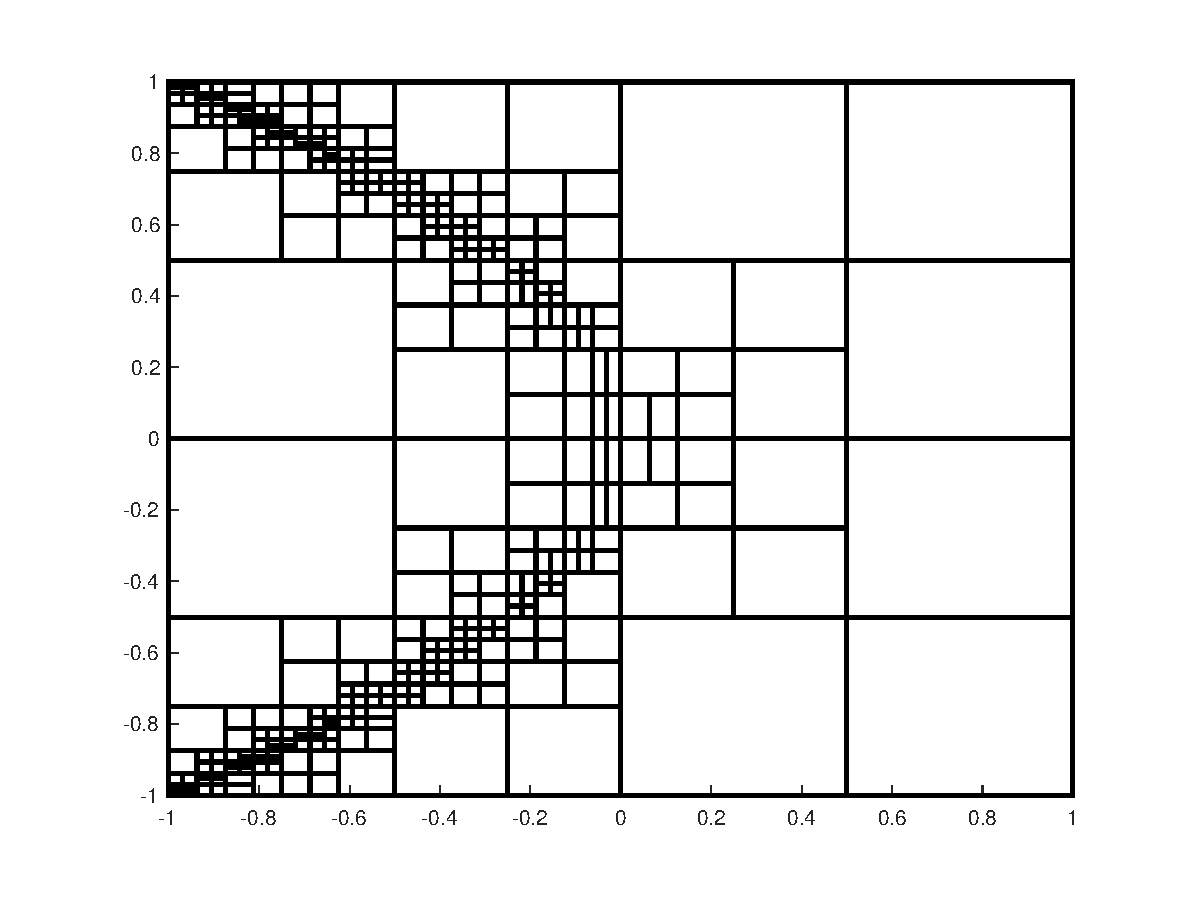
\includegraphics[scale = 0.3]{tan_100_2.eps}
   \label{zone_tan_b}
 }
 
 \subfloat[Zone plot of $f_1(x,y)+f_2(x,y)$]{
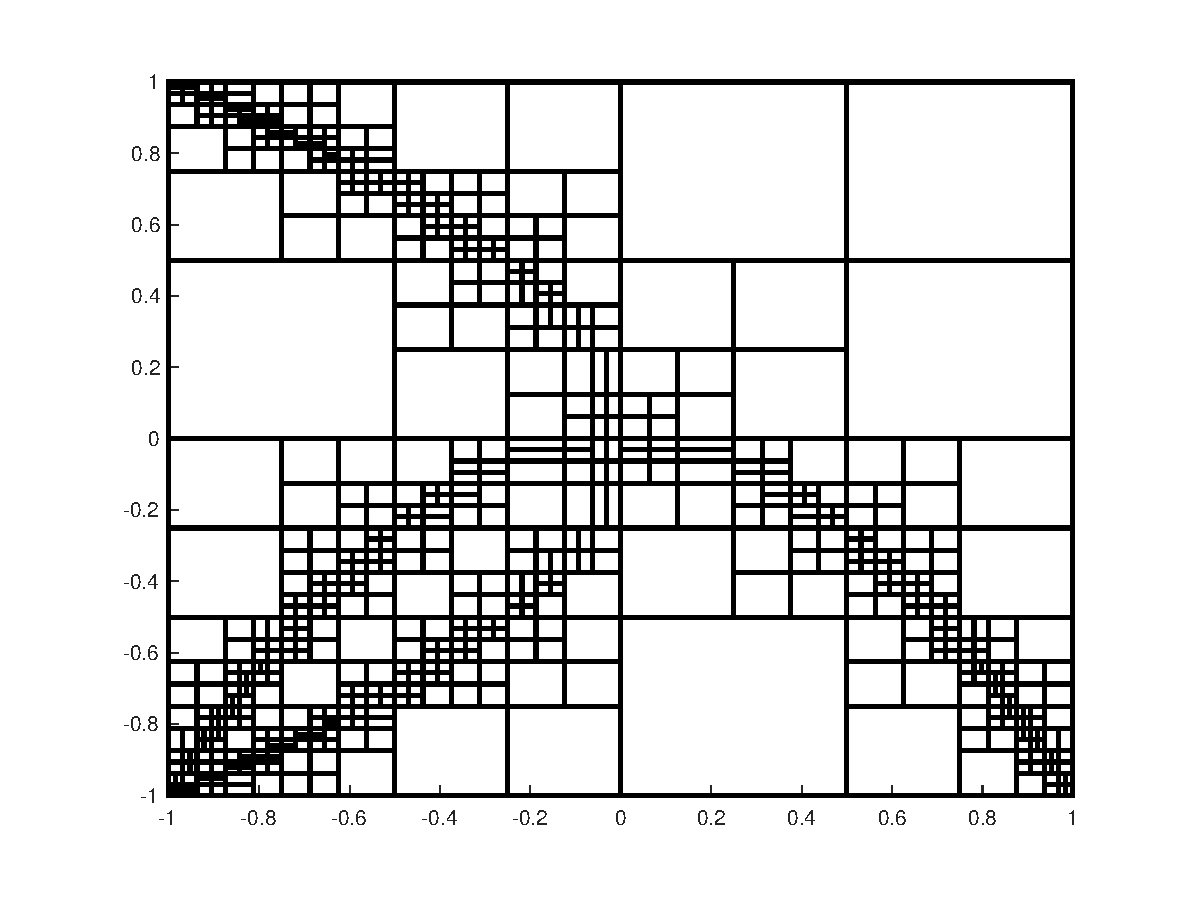
\includegraphics[scale = 0.3]{tan_100_3.eps}
   \label{zone_tan_c}
 }
 \caption{Zone plots for $f_1(x,y)$,$f_2(x,y)$ and $f_1(x,y)+f_2(x,y)$.}
\label{zone_tan}
\end{figure}
 




\subsection{Differentiation}

Differentiation of the global approximant~(\ref{eq:pu-approx}) results in two groups of terms:
\begin{equation}
  \pp{}{x_j} s(\vect{x}) = \sum_{\nu\in \text{leaves}(\ct)} w_\nu(\vect{x}) \pp{}{x_j} s_\nu(\vect{x}) + \sum_{\nu\in \text{leaves}(\ct)} s_\nu(\vect{x}) \pp{}{x_j} w_\nu(\vect{x}).
  \label{eq:pu-deriv}	
\end{equation}
The first sum is a partition of unity approximation of leafwise differentiated interpolants. That is, we simply apply standard spectral differentiation to the data stored in the leaves of $\ct$.

For the second sum, note that the weight function derivatives are nonzero only at values of $\vect{x}$ that lie in the domains of more than one leaf; elsewhere the weight functions are identically one or zero. If the values of all the leafwise interpolants agree perfectly at such $\vect{x}$, then
\begin{equation}
  \label{eq:pu-weight-deriv}
  \sum_{\nu\in \text{leaves}(\ct)} s_\nu(\vect{x}) \pp{}{x_j} w_\nu(\vect{x})
  = s_\nu(\vect{x}) \pp{}{x_j}  \sum_{\nu\in \text{leaves}(\ct)} w_\nu(\vect{x}) = 0,
\end{equation}
since the weights are a partition of unity. Thus this term essentially contributes an amount on the order of the local interpolation accuracy times the gradients of the weights. These are inversely proportional to the overlap widths, which are themselves proportional to the zone widths (see~(\ref{eq:overlap}). At most, then, they contribute an amount that is $\bigo(2^m)$ larger than the original local error on a leaf that is at depth $m$ in the tree. As a practical issue, we are unlikely to be able to cope anyway with a tree of depth great enough to incur a factor as large as two full orders of magnitude---which we would need only to resolve features at a scale much less than 1\% of the original domain width. Hence we feel justified ignoring this contribution. 


\subsection{Integration}

The simplest and seemingly most efficient approach to integrating over the domain is to do so piecewise over the nonoverlapping zones,
\begin{equation}
  \label{eq:integration}
  \int_{\Omega} f(\vect{x}) d\vect{x} = \sum_{\nu\in \text{leaves}(\ct)} \int_{\text{\textsf{zone}($\nu$)}} f(\vect{x}) d\vect{x}.
\end{equation}
Since the leaf interpolants are defined natively over the overlapping domains, they must be resampled at Chebyshev grids on the zones, after which Clenshaw-Curtis quadrature is applied.

\section{Numerical experiments}
\label{sec:numerical_experiments}

All the following experiments were performed on a computer with a 2.6 GHz Intel Core i5 processor in version 2017a of MATLAB. Our code, which uses a serial object-oriented recursive implementation of the algorithms, is available for download at ??. Comparisons to Chebfun2 and Chebfun3 were done using Chebfun version ??. We also tried to use the Sparse Grid Interpolation Toolbox~\cite{Klimke2005}, but on all the examples we were unable to get it close to our desired error tolerances within its hard-coded limits on sparse grid depth. 

\subsection{2D experiments}

We first test the 2D functions $\log(1+(x^2+y^4)/10^{-5})$, $\arctan((x+y^2)/10^{-2})$, $\frac{10^{-4}}{(10^{-4}+x^2)(10^{-4}+y^2)}$, Franke's function \cite{franke1979critical}, and the smooth functions from the Genz family test package \cite{genz1987package}. For each function we record the time of construction, the time to evaluate on a 200x200 grid, and the max observed error on this grid. 

Table~\ref{putable} shows the results for the new method. For comparison, Table~\ref{chb2table} shows the results for Chebfun2~\cite{townsend2013extension} using version 5.5.0 of Chebfun. For the low-rank test cases, the methods are comparable, with neither showing a consistent advantage; most importantly, both methods are fast. In the tests of high-rank functions, our method enjoys a clear advantage in both construction and evaluation times. Moreover, the method remains fast enough for interactive computing even as the total number of nodes exceeds 1.6 million.  We present plots of the functions and adaptively generated subdomains for the first three test functions in Figures~\ref{TANFUN1}-\ref{rungeFUN1}.



\begin{table}[p]

\begin{tabular}{r|c|c|c|c|c|c}
Function & method & error & construct time & eval time & int time & points \\[5pt] \hline
  \multirow{2}{*}{$\log(1+\frac{x_1^2+x_2^4}{10^{-5}})$} &  tree-based & 1.05$\times 10^{-13}$ & 0.6403 & 0.063 & 0.081 & 110496 \\
  & Chebfun2 & 1.14$\times 10^{-6}$ & 2.2997 & 0.1045 & 0.004 & 30 \\ \hline
  \multirow{2}{*}{$\arctan(\frac{x_1+x_2^2}{10^{-2}})$} & tree-based & 2.15$\times 10^{-12}$ & 2.9690 & 0.3138 & 0.528 & 1553816 \\
  & Chebfun2 & 7.09$\times 10^{-12}$ & 150.2228 & 4.979 & 0.017 & 816 \\ \hline
  \multirow{2}{*}{$\frac{10^{-4}}{(10^{-4}+x_1^2)(10^{-4}+x_2^2)}$} & tree-based & 1.01$\times 10^{-11}$ & 0.7298 & 0.1087 & 0.093 & 145280 \\
  & Chebfun2 & 5.44$\times 10^{-15}$ & 0.0493 & 0.0037 & 0.001 & 1 \\ \hline
  \multirow{2}{*}{franke} & tree-based & 4.22$\times 10^{-15}$ & 0.0116 & 0.0045 & 0.007 & 16641 \\
  & Chebfun2 & 1.33$\times 10^{-15}$ & 0.0198 & 0.0024 & 0.001 & 4 \\ \hline
  \multirow{2}{*}{$\cos(u_1\pi + \sum_{i=1}^2 a_i x_i)$} & tree-based & 2.65$\times 10^{-14}$ & 0.0127 & 0.0025 & 0.002 & 1089 \\
  & Chebfun2 & 4.47$\times 10^{-14}$ & 0.0155 & 0.002 & 0.001 & 2 \\ \hline
  \multirow{2}{*}{$\prod_{i=1}^2 (a_i^{-2}+(x_i-u_i)^2)^{-1}$} & tree-based & 5.00$\times 10^{-12}$ & 0.0555 & 0.016 & 0.011 & 29283 \\
  & Chebfun2 & 1.59$\times 10^{-12}$ & 0.0203 & 0.0022 & 0.001 & 1 \\ \hline
  \multirow{2}{*}{$(1+\sum_{i=1}^2 a_i x_i)^{-3}$} & tree-based & 2.27$\times 10^{-12}$ & 0.0119 & 8.97$\times 10^{-4}$ & 0.001 & 25 \\
  & Chebfun2 & 2.27$\times 10^{-12}$ & 0.0117 & 0.0021 & 0.001 & 4 \\ \hline
  \multirow{2}{*}{$\exp(-\sum_{i=1}^2 a_i^2 (x_i-u_i)^2)$} & tree-based & 1.65$\times 10^{-14}$ & 0.0130 & 0.0026 & 0.002 & 2145 \\
  & Chebfun2 & 4.44$\times 10^{-16}$ & 0.0149 & 0.0022 & 0.001 & 1 
\end{tabular}
\caption{Observed error and wall-clock time for the tree method to construct tree-based and Chebfun2 approximations with target tolerance $10^{-12}$ and $\nmax=129$, and to evaluate it on a 200x200 uniform grid. Also shown is the total number of sampled function values stored over all the leaves of the tree. Here $u=[0.75,0.25]$, and $a=[5,10]$.}
\label{putable}
\end{table}


\begin{figure}
  \centering
  \subfloat[$\arctan \lp (x+y^2)/0.01 \rp$]{
    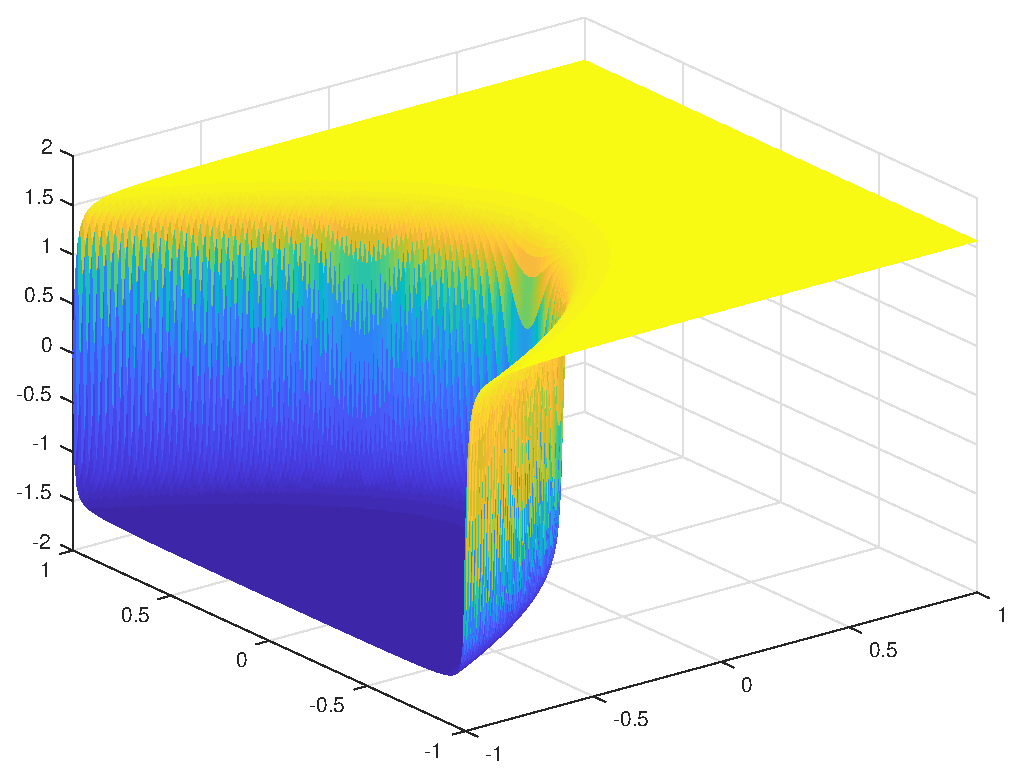
\includegraphics[scale = 0.34]{tan2Dplot}
    \label{tanfunplot}
  }
  \subfloat[Overlapping subdomains]{
    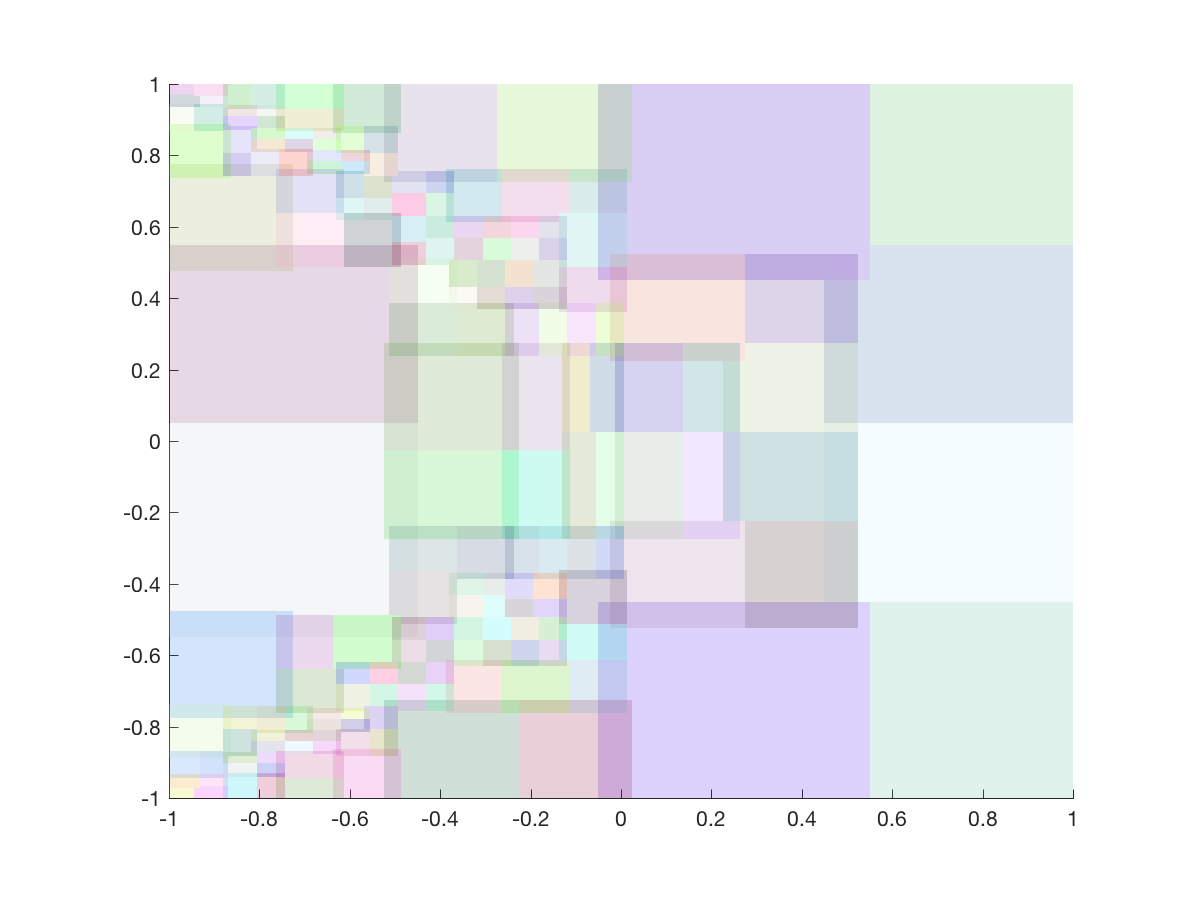
\includegraphics[scale = 0.34]{tan2Dsubdomains}
    \label{tanfundomains}
  }
  \caption{Overlapping subdomains constructed by the adaptive tree method for a function with a nonlinear ``cliff.''}
  \label{TANFUN1}
\end{figure}

\begin{figure}
  \centering
  \subfloat[$\frac{10^{-4}}{(10^{-4}+x^2)(10^{-4}+y^2)}$]{
    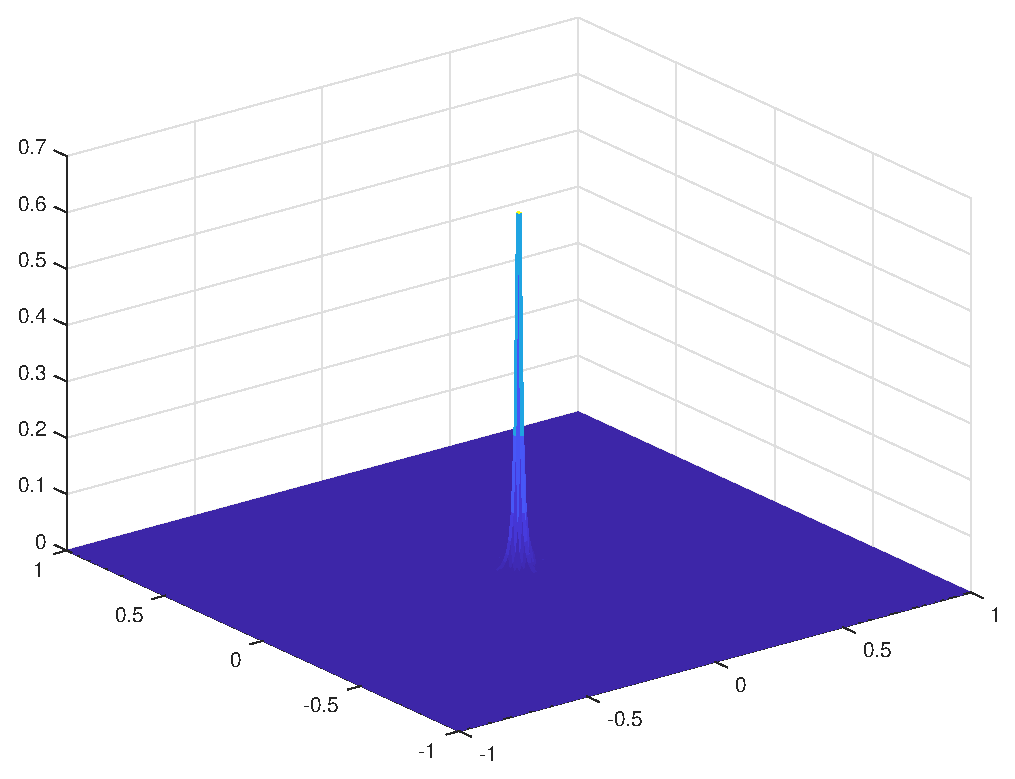
\includegraphics[scale = 0.34]{runge2Dplot}
    \label{rungefunplot}
  }
  \subfloat[Overlapping subdomains]{
    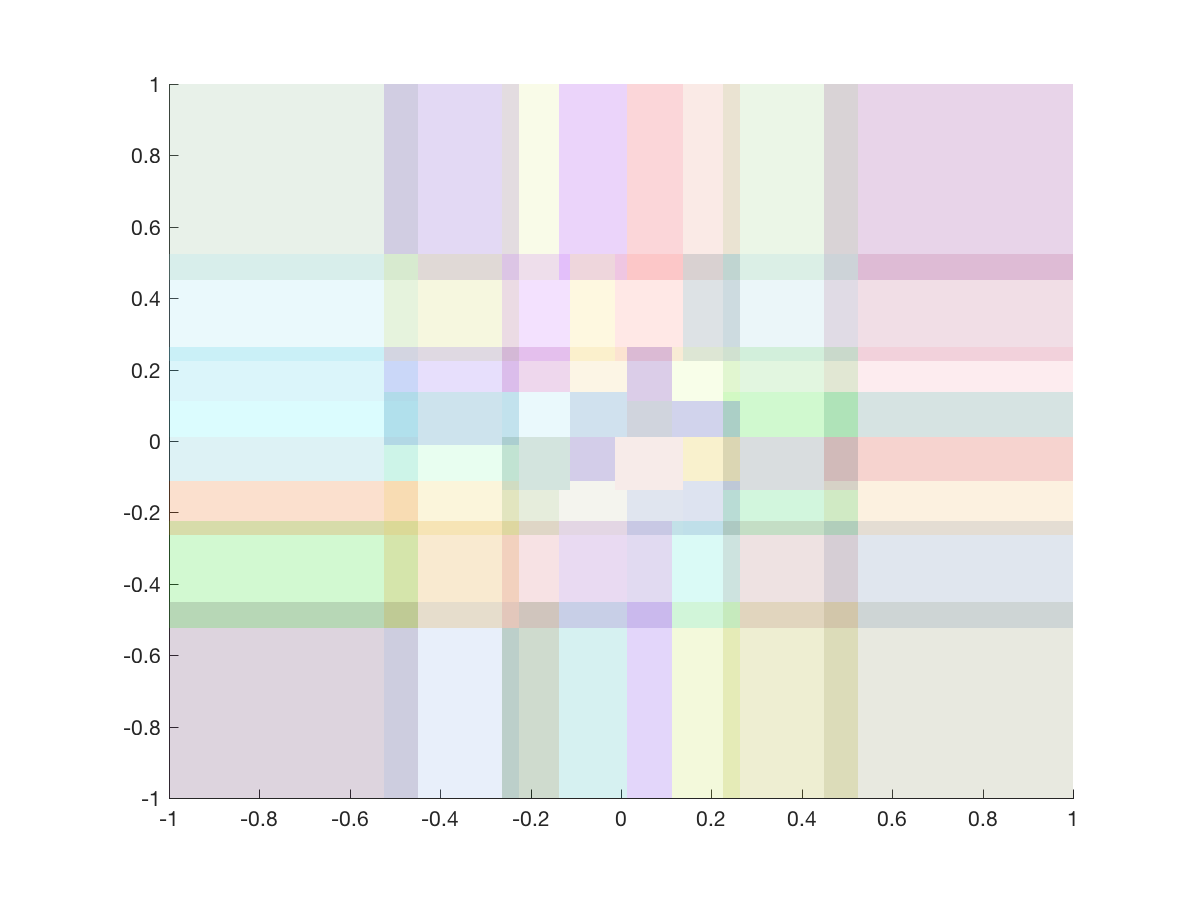
\includegraphics[scale = 0.34]{rungesubdomains}
    \label{rungefundomains}
  }
  \caption{Overlapping subdomains constructed by the adaptive tree method for a function with a sharp spike.}
  \label{rungeFUN1}
\end{figure}


One important aspect of low-rank approximation is that it is inherently nonisotropic. Consider the 2D ``plane wave bump'' 
\begin{equation}
f(x,y)=\arctan(250(\cos(t)x+\sin(t)y))
\label{rotate_func_2D}	
\end{equation}
whose normal makes an angle $t$ with the positive $x$-axis. 
for. We compare the construction times of our method to Chebfun2 for $t \in [0,\pi/4]$ in Figure~\ref{tan_rotate_2D}. We observe the execution time of Chebfun2 varying over nearly three orders of magnitude. While our method is also responsive to the angle of the wave, the variation in time is about half an order of magnitude, and our codes are faster in all but the rank-one case $t=0$ (for which both methods are fast). 


\begin{figure}
\centering
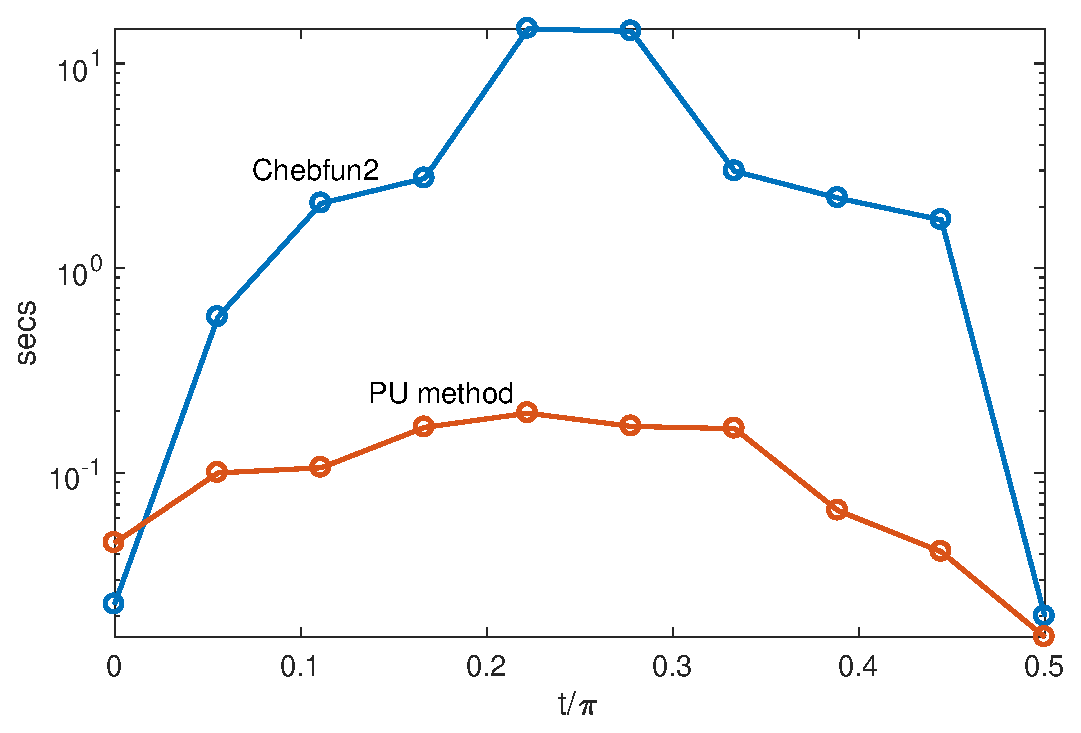
\includegraphics[scale = 0.5]{tan_rotate_2D}
\caption{Comparison of construction times for $\arctan(250(\cos(t)x+\sin(t)y))$ for $t \in [0,\pi/4]$.}
\label{tan_rotate_2D}
\end{figure}


Our next experiment is to add and multiply the rank-one function $\arctan(250x)$ to the plane wave in~(\ref{rotate_func_2D}). The construction time results are compared for $t \in [0,\pi/2]$ in Figure~\ref{TAN_ADD_MULT}. Here the dependence of Chebfun2 on the angle is less severe than in the simple construction, though it is still more pronounced than for our method. More importantly, the absolute numbers for addition in particular with Chebfun2 would probably be considered unacceptable for interactive computation, while our method takes one second at most. 

\begin{figure}
\centering
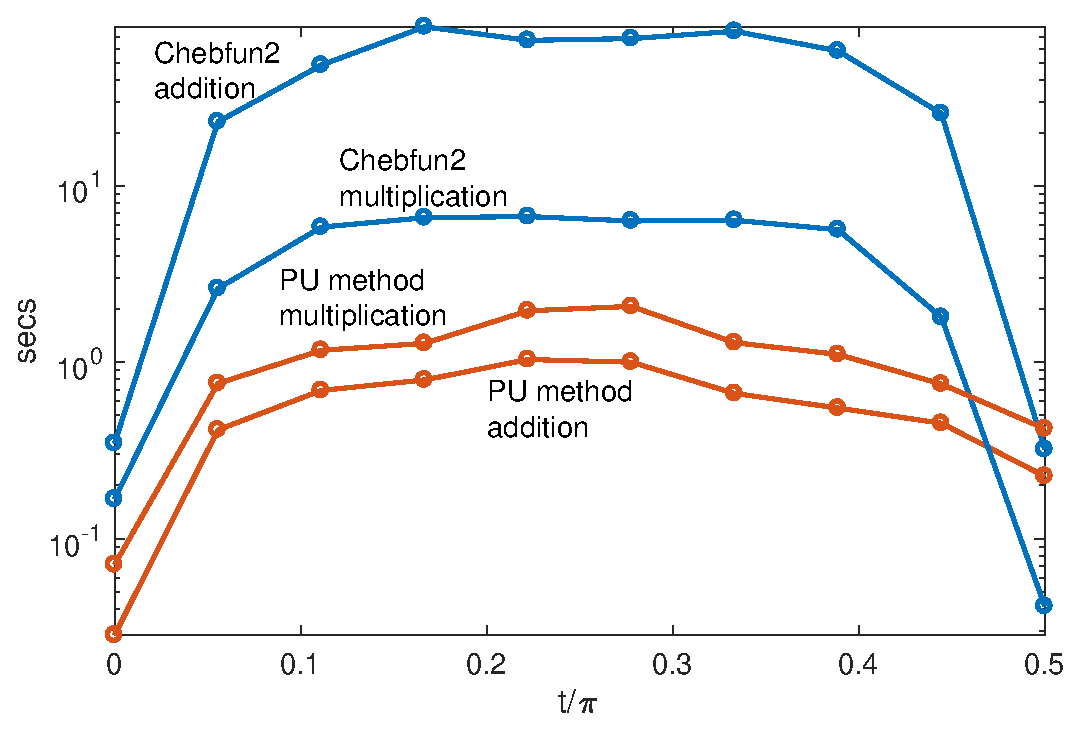
\includegraphics[scale = 0.5]{tan_rotate_add_mult_2D}
\caption{Comparison of execution times for multiplication and addition of $\arctan(250x)$ with $\arctan(250(\cos(t)x+\sin(t)y))$ for $t \in [0,\pi/4]$.}
\label{TAN_ADD_MULT}
\end{figure}



% \begin{figure}
% \centering
% \subfloat[Plot of $\log(1+(x^2+y^4)/10^{-5})$.]{
% 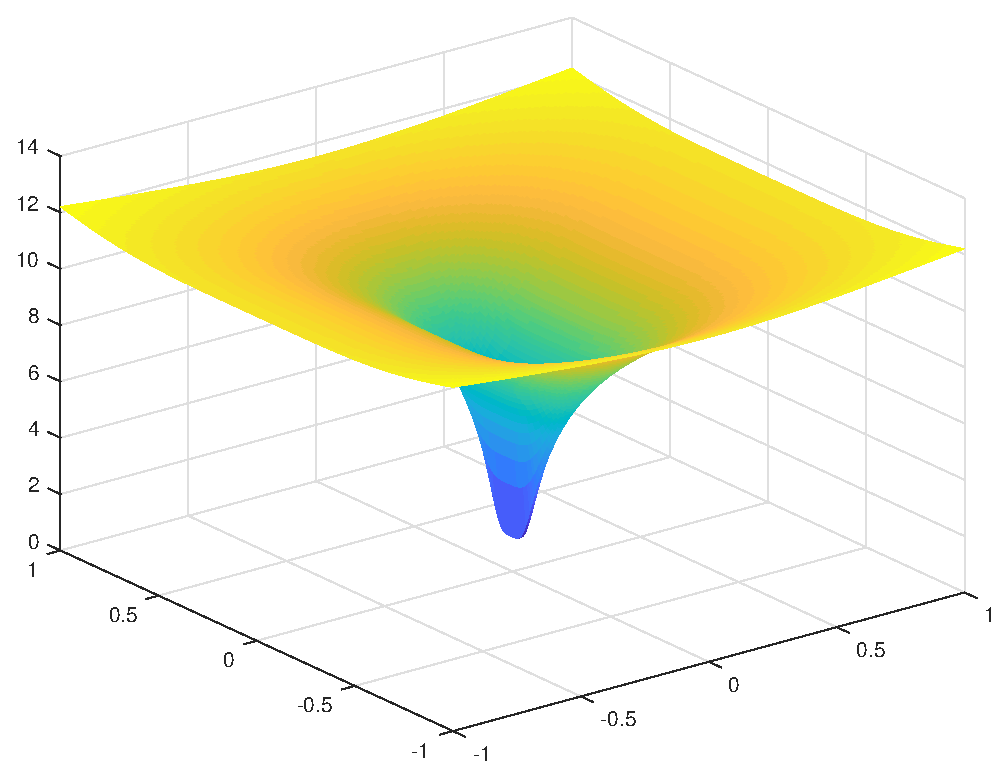
\includegraphics[scale = 0.34]{log2Dplot.eps}
%    \label{logfunplot}
%  }
% \subfloat[Plot of subdomains.]{
% 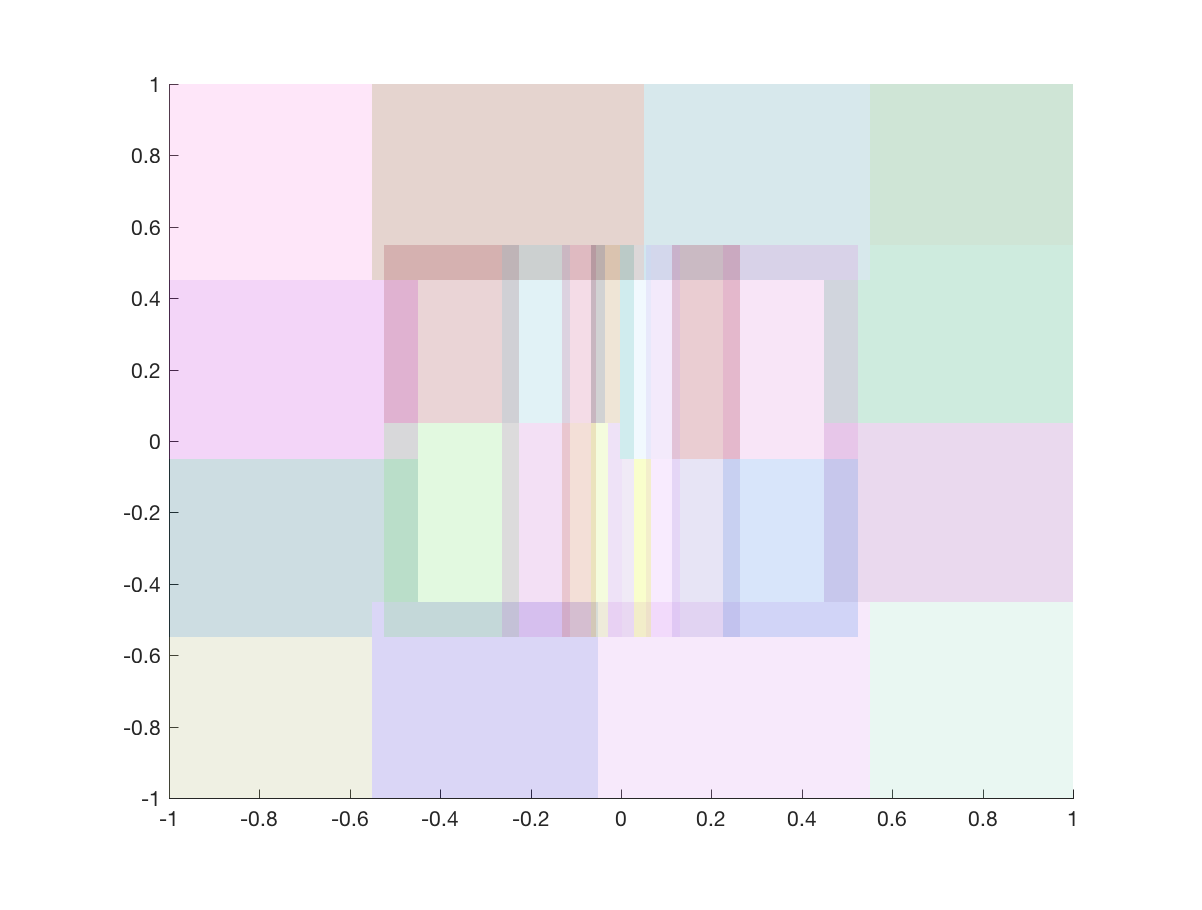
\includegraphics[scale = 0.34]{log2Dsubdomains.eps}
%    \label{logfundomains}
%  }
% \caption{Plot of $\log(1+(x^2+y^4)/10^{-5})$ and the subdomains formed from the partition of unity method.}
% \label{logFUN1}
% \end{figure}


\subsection{3D experiments}

We next test the 3D functions $1/(\cosh(5(x+y+z)))^2$, $\arctan(5(x+y)+z)$, and 3D versions of the smooth functions from the Genz family test package. We similarly record the construction time, time to evaluate on a $200\times 200 \times 200$ grid and the max error on the grid.

Results for the tree-based method and Chebfun3 are presented in Tables~\ref{putable3D}--\ref{chb3table}. We see that Chebfun3 performs well for low-rank functions,\footnote{In Chebfun3, functions are approximated in a compressed splice-Tucker decomposition, a variant of a multivariate adaptive cross approximation \cite{bebendorf2011adaptive}. Here rank refers to the so-called Tucker rank.}, outperforming the tree-based method in construction time in those cases, with more mixed results for evaluation times. However, the tree-based method is still operating within acceptable interactive speed in these cases. We also note that in case, both methods failed to get close to the targeted accuracy.

For the two higher-rank examples, the story is very different. The tree-based method is able to perform all the tests in under a second, while Chebfun3 requires over 80 seconds to construct these cases. Once Chebfun3 finds the approximation, its evaluation time is also under a second.  


\begin{table}[p]
\begin{tabular}{r|c|c|c|c}
& error & construct time & eval time & points \\[5pt] \hline
$\cos(u_1\pi + \sum_{i=1}^3 a_i x_i)$ & 22.71$\times 10^{-14}$ & 0.151 & 0.118 & 275000 \\ [5pt]
$\prod_{i=1}^3 (a_i^{-2}+(x_i-u_i)^2)^{-1}$ & 1.52$\times 10^{-5}$ & 7.204 & 1.312 & 10400000 \\[2pt]
$(1+\sum_{i=1}^3 a_i x_i)^{-3}$ & 4.66$\times 10^{-10}$ & 0.16555 & 0.033 & 125 \\[5pt]
$\exp(-\sum_{i=1}^2 a_i^2 (x_i-u_i)^2)$ & 3.11$\times 10^{-15}$ & 0.0818 & 0.078 & 275000  \\[5pt]
$1/(\cosh(5(x+y+z)))^2$ & 1.14$\times 10^{-14}$ & 0.706 & 0.545 & 2200000 \\
$\arctan(5(x+y)+z)$ & 7.60$\times 10^{-13}$ & 0.7512 & 0.030 & 549153 \\
\end{tabular}
\caption{Observed error and wall-clock time for the tree method to construct a tree approximation with target tolerance $10^{-12}$ and $\nmax=65$, and to evaluate it on a 200$^3$ uniform grid. Also shown is the total number of sampled function values stored over all the leaves of the tree. Here $u=[0.75,0.25,-0.75]$ and $a=[25,25,25]$.}
\label{putable3D}
\end{table}

\begin{table}[p]
\begin{tabular}{r|c|c|c|c}
& error & construct time & eval time & rank \\[5pt] \hline
$\cos(u_1\pi + \sum_{i=1}^2 a_i x_i)$ & 2.16$\times 10^{-14}$ & 0.061 & 0.150 & 2  \\[5pt]
$\prod_{i=1}^2 (a_i^{-2}+(x_i-u_i)^2)^{-1}$ & 5.66$\times 10^{-7}$ & 0.057 & 0.137 & 1 \\[5pt]
$(1+\sum_{i=1}^2 a_i x_i)^{-3}$ & 4.07$\times 10^{-10}$ & 0.038 & 0.143 & 4 \\[5pt]
$\exp(-\sum_{i=1}^2 a_i^2 (x_i-u_i)^2)$ & 7.77$\times 10^{-16}$ & 0.047 & 0.144 & 1 \\[5pt]
$1/(\cosh(5(x+y+z)))^2$ & 3.69$\times 10^{-13}$ & 80.666 & 0.398 & 93 \\
$\arctan(5(x+y)+z)$ & 4.69$\times 10^{-13}$ & 89.957 & 0.104 & 110 \\
\end{tabular}
\caption{Observed error and wall-clock time for Chebfun3 using default settings to construct an approximation and evaluate it on a 200$^3$ uniform grid. Also shown is the computed rank of the function. Here $u=[0.75,0.25,-0.75]$ and $a=[25,25,25]$.}	
\label{chb3table}
\end{table}

We repeat our experiment testing the importance of axes alignment using the function
\begin{equation}
\arctan(5(\sin(p)\cos(t)x+\sin(p)\sin(t)y+\cos(p)z))
\end{equation}
for $p,t \in [0,\pi/4]$. Timing results can be seen in Figure~\ref{fig:tan3D}. As in 2D, the Chebfun low-rank technique shows wide variation depending on the angles, and a large region of long times. The tree-based method is much less sensitive and faster (by as much as two orders of magnitude) except for the purely axes-aligned cases. 

\begin{figure}
  \centering
  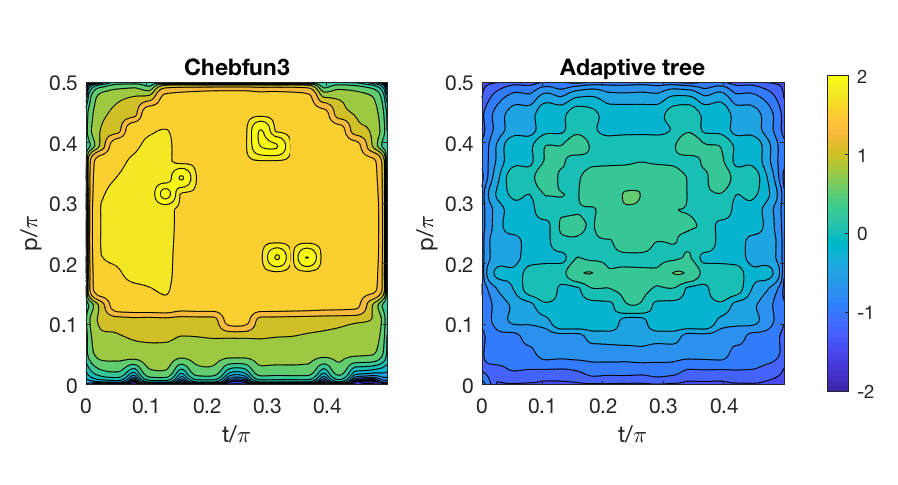
\includegraphics[width=\textwidth]{tan3d_comparison}
  \caption{Construction time comparison for the 3D function $\arctan(5(\sin(p)\cos(t)x+\sin(p)\sin(t)y+\cos(p)z))$, with varying angles. Colors and contours correspond to the base-10 log of execution time in seconds.}
  \label{fig:tan3D}
\end{figure}

\section{Extension to nonrectangular domains}

We now consider approximation over a nonrectangular domain $\Omega\subset \R^d$. In our construction, a leaf node $\nu$ whose domain $\Omega_\nu$ lies entirely within $\Omega$ can be treated as before. However, if $\Omega_\nu\cap \Omega \subsetneq \Omega_\nu$, we need a different approximation technique on $\nu$. We will again select a tensor-product Chebyshev polynomial as in~(\ref{eq:full-interp}), but choose its coefficient array $C$ by satisfying a discrete least squares criterion:
\begin{equation}
  \argmin_{C} \sum_{i=1}^{P} \lp f(\vect{x}_i) -  \tilde{p}(\vect{x}_i) \rp^2,
\end{equation}
where $\Xi = \{\vect{x}_i\}_{i=1}^{P} \subset \Omega_\nu\cap \Omega$ is a point set in the ``active'' part of the leaf's domain, $\Omega_\nu\cap \Omega$. In practice we can form a matrix $A$ whose columns are evaluations of each basis function at the points in $\Xi$, leading to a standard $P\times N^d$ linear least squares problem. We choose $\Xi$ as the part of the standard $(2N)^d$-sized Chebyshev grid lying inside $\Omega$. 

This technique resembles Fourier extension or continuation techniques~\cite{adcock2014resolution,adcock2014numerical,huybrechs2010fourier}, so we refer to it as a \emph{Chebyshev extension approximation}. Unlike the Fourier case, however, there is no real domain extension involved; rather one constrains the usual multivariate polynomial only over part of its usual tensor-product domain. The condition number of $A$ in the discrete Fourier extension case has been shown to increase exponentially with the degree of the approximation \cite{adcock2014numerical}, but we expect to avoid having problems with this by capping $N$ and subdividing the domain instead.

We modify Algorithm~\ref{alg:split} so that when a domain is split, the resulting zones of the children are shrunk if possible to just contact the boundary of $\Omega$. (An exception is the shared interface between the newly created children, which is fixed.) This helps to keep a substantial proportion of a leaf's domain within $\Omega$.

We also modify how refinement decisions are made and executed in Algorithm~\ref{alg:refine}, for a subtle reason. The original algorithm is able to exploit the very different resolution requirements for a function such as, say, $xT_{60}(y)$, by testing for sufficient resolution in each dimension independently and splitting accordingly. We find experimentally that if the function is like this over $\Omega$, the extension of it to the unconstrained part of the leaf node's domain has uniform resolution needs in all variables. Therefore, we use a simpler refinement process: if the norm of the least-squares residual (normalized by $\sqrt{P}$) is not acceptably small, we split in all dimensions successively. In effect, the approximation becomes a quadtree or octree within those leaves that do not lie entirely within $\Omega$. 


% \begin{algorithm}
% \caption{split($\Omega$,$\nu$,$j$,$t$)}
% \label{alg:LSsplit}
% \begin{algorithmic}
% \IF{$\nu$ is a leaf}
% \STATE \textsf{splitdim}($\nu$)=$j$
% \STATE Define new nodes $\nu_0$, $\nu_1$
% \STATE $[a_1,b_1],[a_2,b_2],\dots,[a_n,b_n]$ be the subintervals from \prop{zone}{$\nu$}
% \STATE Let $m:= \frac{b_j+a_j}{2}$
% \STATE Let \textsf{zone}($\nu_0$) $:= [a_1,b_1] \times \dots \times [a_{j-1},b_{j-1}] \times [a_{j},m] \times [a_{j+1},b_{j+1}] \times \dots \times [a_{d},b_{d}] $
% \STATE Let \textsf{zone}($\nu_1$) $:= [a_1,b_1] \times \dots \times [a_{j-1},b_{j-1}] \times [m,b_{j}] \times [a_{j+1},b_{j+1}] \times \dots \times [a_{d},b_{d}] $
% \FOR{$k=0,1$}
% \STATE Define \textsf{domain}($\nu_k$) from \textsf{zone}($\nu_k$) with parameter $t$ as in~(\ref{eq:zone_extend})
% \IF{$\text{\textsf{domain}($\nu_k$)} \cap \Omega = \emptyset$}
% \STATE $\nu_k$ = NULL
% \ELSIF{$\text{\textsf{domain}($\nu_k$)} \subseteq \Omega$}
% \STATE define $\nu_k$ as node on a hypercube.
% \ELSE
% \STATE For dimensions $p=1,2,\dots,j-1,j+1,\dots,d$ change subintervals $[a_p,b_p]$ of \textsf{domain}($\nu_k$) and \textsf{zone}($\nu_k$) to fit $\Omega$.
% \STATE For dimension $p=j$, change subinterval $[a_p,b_p]$ of \textsf{domain}($\nu_k$) by choosing largest $a_p$ such that $\Omega \subset \text{\textsf{domain}($\nu_k$)}$ if $k=0$, and vice versa if $k=1$. Change endpoints of \textsf{zone}($\nu_k$) to match changed endpoints of \textsf{domain}($\nu_k$).
% \ENDIF
% \STATE Define \textsf{grid}($\nu_k$) as Chebyshev tensor-product grid of size $\nmax^d$ in \textsf{domain}($\nu_k$)
% \STATE Let \textsf{isdone}($\nu_k$):= \textsf{isdone}($\nu$)
% \ENDFOR
% \ELSE
% \STATE split(\child{0}($\nu$),$k$,$t$)
% \STATE split(\child{1}($\nu$),$k$,$t$)
% \ENDIF
% \end{algorithmic}
% \end{algorithm}

\subsection{Numerical experiments}

For the 2D Chebyshev extension method we test
\begin{equation}
  \label{eq:testfun-gen}
  \begin{aligned}
    g_1& =\exp(x+y), & g_2&=\dfrac{1}{((x-1.1)^2)+(y-1.1)^2)^2}, \\
    g_3 &=\cos(24x-32y)\sin(21x-28y), & g_4&=\arctan(3(x^2+y)).
  \end{aligned}
\end{equation}
We approximated each function on each of three domains: the unit disk, the diamond $|x|+|y|\le 1$, and the double astroid seen in Figure~\ref{star_plot}. The initial box (root of the approximation tree) was chosen to tightly enclose the given domain. For each test we set $N=17$ and the target tolerance to $10^{-10}$
We timed both the adaptive construction and the evaluation on a $200\times 200$ grid, and recorded the max error as in the previous section. In each case, we choose initial box to fit the domain as tightly as possible. These results can be seen in Tables~\ref{table_general}. The resulting approximation of $g_4$ on the double astroid is shown in Figure~\ref{star_plot}, along with the adaptively found subdomains. 

We see when the function is smooth or contains localized features, the method is both efficient and highly accurate; in the smoothest case of $g_1$, a global multivariate least-squares polynomial is sufficient. Only for $g_3$, which requires uniformly fine resolution throughout the domains, is there a construction time longer than a few seconds. The Fourier extension methods described in~\cite{matthysen2017function} are implemented in Julia, making a direct quantitative comparisons difficult, but based on the orders of magnitude of the results reported there, we feel confident that our results for these examples are superior. 


% \begin{figure}
% \centering

% \subfloat[Diamond domain]{
% 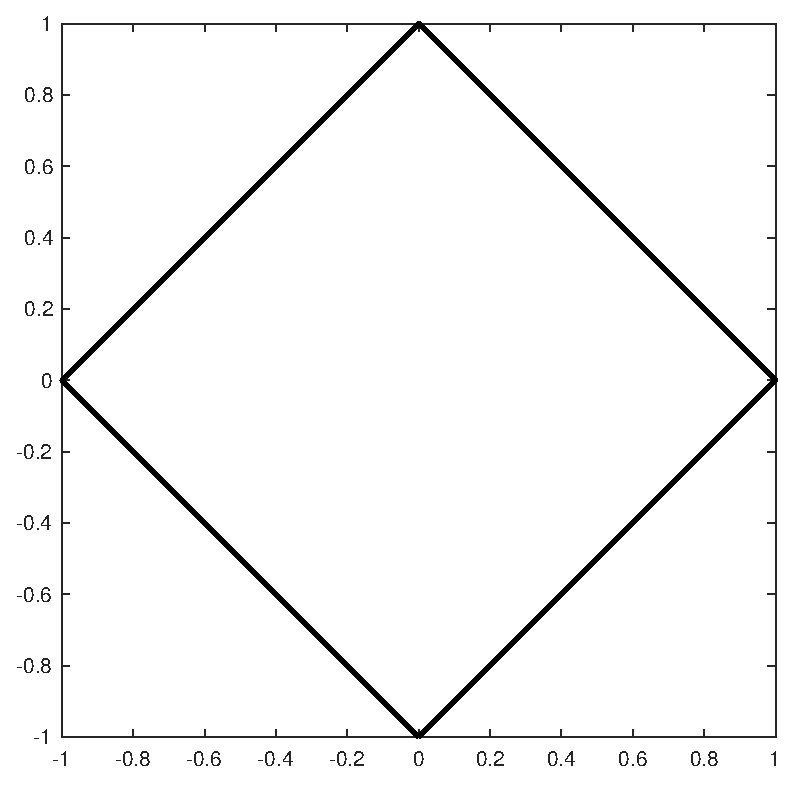
\includegraphics[scale = 0.3]{diamond.eps}
%    \label{domain_b}
%  }
%  \subfloat[Double astroid domain]{
% 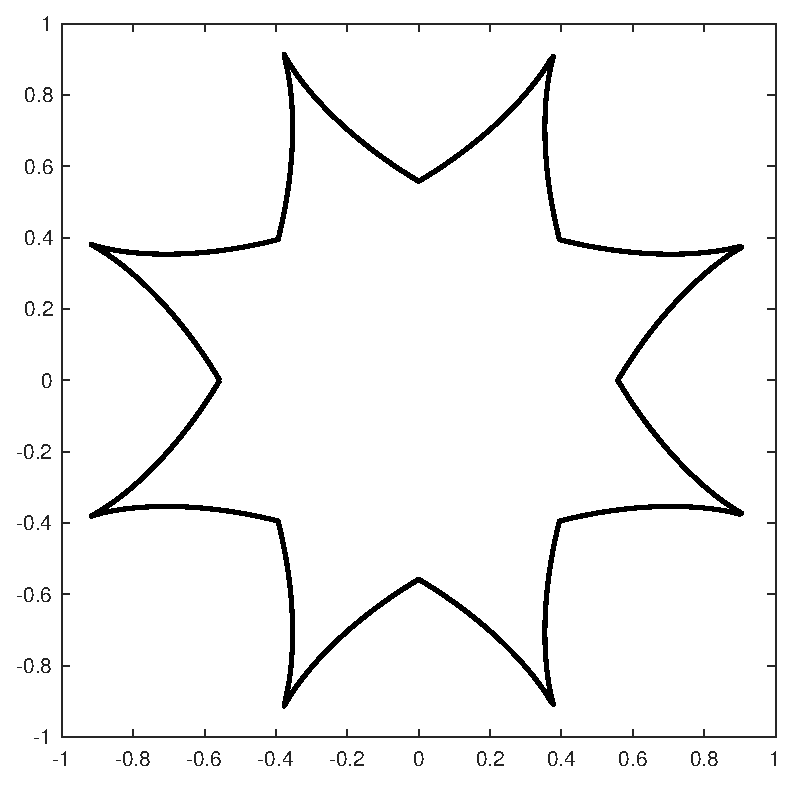
\includegraphics[scale = 0.3]{star.eps}
%    \label{domain_c}
%  }
%  \caption{Plots of the domains we tested on 2D. The double astroid domain is the union of two rotated astroid curves.}
% \label{domains}
% \end{figure}

\begin{figure}
\centering
\subfloat[Plot of $\arctan(3(y^2+x))$.]{
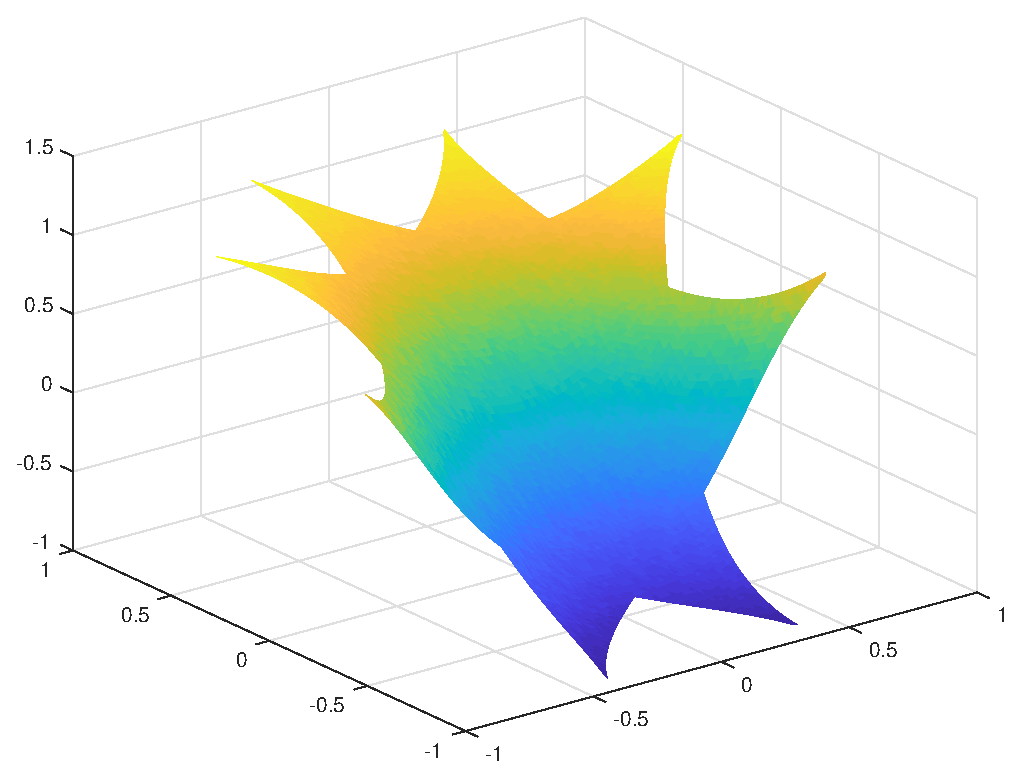
\includegraphics[scale = 0.34]{starPlot.eps}
   \label{star_plota}
 }
\subfloat[Plot of subdomains.]{
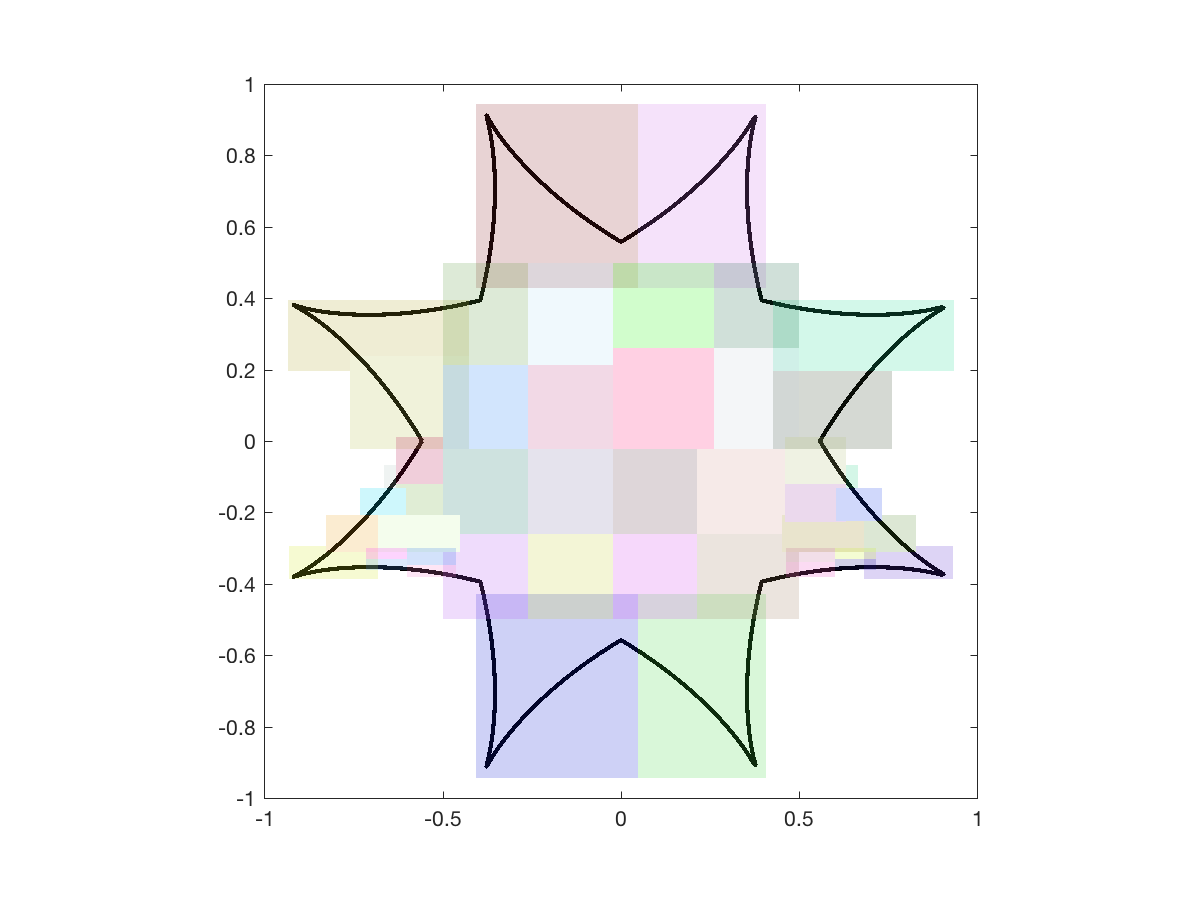
\includegraphics[scale = 0.34]{starPlotDoms.eps}
   \label{star_plotb}
 }
\caption{Plot of $\arctan(3(y^2+x))$ and the subdomains formed from the partition of unity method.}
\label{star_plot}
\end{figure}


\begin{table}
\begin{tabular}{c|c|c|c|c|c}
function & domain & error & construct time & interp time & points \\ [5pt] \hline
\multirow{3}{*}{ $g_1$ } & disk & 5.44E-15 & 1.369 & 0.012 & 289 \\
& diamond & 2.06E-11 & 0.040 & 0.002 & 289 \\
& astroid & 2.01E-08 & 0.071 & 0.001 & 289 \\ \hline
\multirow{3}{*}{ $g_2$ } & disk & 2.40E-10 & 2.558 & 0.117 & 3757 \\
& diamond & 2.40E-11 & 0.406 & 0.012 & 2023 \\
& astroid & 2.14E-10 & 1.511 & 0.023 & 4624 \\ \hline
\multirow{3}{*}{ $g_3$ } & disk & 4.44E-11 & 11.305 & 1.500 & 245650 \\
& diamond & 2.35E-11 & 10.894 & 0.854 & 178020 \\
& astroid & 1.67E-10 & 28.072 & 0.836 & 153780 \\ \hline
\multirow{3}{*}{ $g_4$ } & disk & 7.49E-11 & 1.866 & 0.059 & 12138 \\
& diamond & 1.45E-11 & 1.536 & 0.053 & 9826 \\
& astroid & 1.09E-11 & 3.221 & 0.049 & 9826 \\
\end{tabular}
  \caption{Observed error and wall-clock times for the adaptive tree method to approximate the functions given in~(\ref{eq:testfun-gen}) on three different 2D domains. Also shown is the total number of sampled function values stored over all the leaves of each final tree.}
  \label{table_general}
\end{table}


\section{Concluding remarks}
\label{sec:conclusion}

For functions over hyperrectangles of uncorrelated variables or that otherwise are well-aligned with coordinate axes, low-rank and sparse-grid approximations can be expected to be highly performant. We have demonstrated an alternative approach that, in two or three dimensions, still performs well on such functions but is far less dependent on that property. Our method sacrifices the use of a single global representation that could achieve true spectral convergence, but in practice we are able to use a partition of unity to construct a smooth, global approximation of very high accuracy in a wide range of examples. 

The adaptive domain decomposition offers some other potential advantages we have not yet exploited, but are studying. It offers a built-in parallelism for function construction and evaluation. It allows efficient updating of function values locally, rather than globally, over the domain. It has a built-in preconditioning strategy, based on additive Schwarz methods, for the solution of partial differential equations.

Finally, domain decomposition offers a particular strategy for functions defined over nonrectangular domains. A node in the tree can use the tensor-product polynomial approximation if its rectangular domain lies within the domain of $f$, or something else otherwise. Geometric refinement can then help to significantly mollify the approximation problem. 

\bibliographystyle{siamplain}
\bibliography{PU_BIB}

\begin{appendices}

\section{Merging trees}
\label{sec:merge}

Algorithm~\ref{alg:merge} describes a recursive method for merging two trees $\ct_1$ and $\ct_2$, representing functions $f_1$ and $f_2$, into a tree representation for $f_1\circ f_2$, with $\circ$ as $+$, $-$, $\times$, or $\div$. The input arguments to the algorithm are the operation, corresponding nodes of $\ct_1$, $\ct_2$, and the merged tree, and the number $r$, which is the dimension that was most recently split in the merged tree. Initially the algorithm is called with root nodes representing the entire original domain, and $r=0$. 

We assume an important relationship among the input nodes. Suppose that \prop{zone}{$\nu_k$}=$\prod_{j=1}^d [\alpha_{kj},\beta_{kj}]$ for $k=1,2$, and that \prop{zone}{$\Tm$}=$\prod_{j=1}^d [A_{j},B_{j}]$. Then we require for $k=1,2$ that
\begin{equation}
  \label{eq:merge-zones}
  [a_{kj},b_{kj}]=[A_j,B_j] \quad \text{for all $j$ having} \quad   \prop{isdone}{\nu_k}_j=
  \text{FALSE}.
\end{equation}
This is trivially true at the root level. The significance of this requirement is that it allows us to avoid ambiguity about what the zone of $\Tm$ should be after a new split in, say, dimension $j$. Since only an uncompleted dimension can be split, the zone of the children of \Tm after splitting will be identical to that of whichever (or both) of the $\nu_k$ requires refinement in dimension $j$.

For example, suppose the zones of $\nu_1$ and $\nu_2$ are $[-1,0]\times[-1,1]$ and $[-1,1]\times[0,1]$, respectively, and \prop{zone}{\Tm}=$[-1,0]\times[0,1]$. It's clear that we can interpolate from $\nu_1$ and $\nu_2$ onto \Tm. It's also clear that we can further split in $x$ in $\nu_1$, and in $y$ in $\nu_2$. But if we were to split $\nu_2$ in $x$, one of the children would have zone $[0,1]\times[0,1]$, which is inaccessible to $\nu_1$. 

Consider the general recursive call. If both $\nu_1$ and $\nu_2$ are leaves, then we simply evaluate the result of operating on their interpolants to get the values on \Tm. If exactly one of $\nu_1$ and $\nu_2$ is a leaf, then we split \Tm the same way as the non-leaf and recurse into the resulting children; property~(\ref{eq:merge-zones}) trivially remains true in these calls. If both  $\nu_1$ and $\nu_2$ are non-leaves, and they both split in the same dimension, then we can split $\Tm$ in that dimension and recurse, and the zones will continue to match as in~(\ref{eq:merge-zones}).

The only remaining case is that $\nu_1$ and $\nu_2$ are each split, but in different dimensions. In this case we have to use information about how the splittings are constructed in Algorithm~\ref{alg:refine}. Recall that each unresolved dimension is split in order, while resolved dimensions are flagged as finished in all descendants. By inductive assumption, \Tm was most recently split in dimension $r$. The algorithm determines which $\nu_k$ has splitting dimension $j$ that comes the soonest after $r$ (computed cyclically). Thus for all dimensions between $r$ and $j$, neither of the given nodes splits, so it and its descendants all must have \textsf{isdone} set to TRUE in those dimensions, and property~(\ref{eq:merge-zones}) makes no requirement. Furthermore, the dimension $r_k$ does satisfy~(\ref{eq:merge-zones}) for $\nu_k$, and the same will be true for its children and the children of $\Tm$. All other dimensions will inherit~(\ref{eq:merge-zones}) from the parents. 


\newcommand{\op}{\ensuremath{\circ}}
\begin{algorithm}[!h]
\caption{merge(\op,$\nu_1$,$\nu_2$,$\num$,$r$)}
\label{alg:merge}
\begin{algorithmic}
\IF{$\nu_1$ and $\nu_2$ are leaves}
\STATE \textsf{values}($\num$):= \textsf{interpolant}($\nu_1$) $\op$ \textsf{interpolant}($\nu_2$), evaluated on \prop{grid}{$T_\text{merge}$}
\ELSIF{$\nu_1$ is a leaf \AND $\nu_2$ is not a leaf}
\STATE split($\num$,\prop{splitdim}{$\nu_1$})
\STATE merge(\op,$\nu_1$,\child{0}($\nu_2$),\child{0}($\num$),\prop{splitdim}{$\nu_2$})
\STATE merge(\op,$\nu_1$,\child{1}($\nu_2$),\child{1}($\num$),\prop{splitdim}{$\nu_2$})
\ELSIF{$\nu_1$ is not a leaf \AND $\nu_2$ is a leaf}
\STATE split($\num$,\prop{splitdim}{$\nu_1$})
\STATE merge(\child{0}($\nu_1$),$\nu_2$,\child{0}($\num$),\prop{splitdim}{$\nu_1$})
\STATE merge(\child{1}($\nu_1$),$\nu_2$,\child{1}($\num$),\prop{splitdim}{$\nu_1$})
\ELSE
\IF{\prop{splitdim}{$\nu_1$}=\prop{splitdim}{$\nu_2$}}
\STATE split($\num$,\prop{splitdim}{$\nu_1$})
\STATE merge(\op,\child{0}($\nu_1$),\child{0}($\nu_2$),\child{0}($\num$),\prop{splitdim}{$\nu_1$})
\STATE merge(\op,\child{1}($\nu_1$),\child{1}($\nu_2$),\child{1}($\num$),\prop{splitdim}{$\nu_1$})
\ELSE
\STATE $r_1 = (\text{\prop{splitdim}{$\nu_1$}}-r-1) \mod d$
\STATE $r_2 = (\text{\prop{splitdim}{$\nu_2$}}-r-1) \mod d$
\STATE If $r_1>r_2$, swap $\nu_1$ and $\nu_2$
\STATE split($\Tm$,\prop{splitdim}{$\nu_1$})
\STATE merge(\op,\child{0}($\nu_1$),$\nu_2$,\child{0}($\num$),\prop{splitdim}{$\nu_1$})
\STATE merge(\op,\child{1}($\nu_1$),$\nu_2$,\child{1}($\num$), \prop{splitdim}{$\nu_1$})
\ENDIF
\ENDIF
\end{algorithmic}
\end{algorithm}




%\begin{theorem}
%Algorithm~\ref{addition3} produces a tree $T_{\text{add}}$ with a merged splitting of $\nu_1$ and $\nu_2$.
%\label{split_theorem_2}
%\end{theorem}
%
%\begin{proof}
%Suppose we have that \textsf{zone}($T_{\text{add}}$) and \textsf{zone}($\nu_1$) are the same along the first dimension i.e. if \textsf{zone}($T_{\text{add}}$)=$[a,b]\times[c,d]$ and \textsf{zone}($\nu_1$)=$[e,f]\times[g,h]$ then $[a,b]=[e,f]$. Then it is clear that if $\nu_1$ and $T_{\text{add}}$ split first in $x$ that \textsf{zone}(\child{k}($T_{\text{add}}$)) and \textsf{zone}(\child{k}($\nu_1$)) will match along the first dimension as well. Suppose for induction that for $k=0,1$ \textsf{zone}($T_{\text{add}}$) and \textsf{zone}($T_k$) are the same along dimensions that $T_k$ still splits in. This is trivially true at the first call since at the root \textsf{zone}($T_{\text{add}}$)=\textsf{zone}($\nu_1$)=\textsf{zone}($\nu_2$).
%
%Suppose we are at a case where $\nu_1$ is not a leaf and we split \textsf{zone}($T_{\text{add}}$) along \textsf{splitdim}($\nu_1$). By the induction hypothesis we have that \textsf{zone}($T_{\text{add}}$) matches \textsf{zone}($\nu_1$) along dimension \textsf{splitdim}($\nu_1$); this gives us that \textsf{zone}(\child{k}($T_{\text{add}}$)) and \textsf{zone}(\child{k}($\nu_1$)) match along \textsf{splitdim}($\nu_1$) as well. Since nothing has changed for the other dimensions, the induction hypothesis holds for \child{k}($\nu_1$) and \child{k}($T_{\text{add}}$).
%
%The only case left is where $\nu_1$ and $\nu_2$ are not leaves, but \textsf{splitdim}($\nu_1$) and \textsf{splitdim}($\nu_2$) differ. Suppose that in this case $nextsplit$=\textsf{splitdim}($\nu_1$) in Algorithm~\ref{addition3}. We then call add(\child{k}($\nu_1$),$\nu_2$,\child{k}($T_{\mbox{add}}$),$nextsplit$). The induction hypothesis holds for \child{k}($\nu_1$) and \child{k}($T_{\mbox{add}}$) for similar reasons as before. Given that \child{k}($T_{\mbox{add}}$) is changed only in \textsf{splitdim}($\nu_1$), the induction hypothesis holds for $\nu_2$ and \child{k}($T_{\mbox{add}}$) for all dimensions except possibly \textsf{splitdim}($\nu_1$). But by Lemma~\ref{split_theorem}, we have $\nu_2$ does not split in \textsf{splitdim}($\nu_1$) so the induction hypothesis holds for $\nu_2$ and \child{k}($T_{\mbox{add}}$).
%\end{proof}


\end{appendices}


%\section{Adaptive alternating Schwarz}
%The \textit{alternating Schwarz method} is an iterative method used to solve boundary value problems. Suppose we wish to solve
%\begin{equation}
%\label{pde_2_solve}
%\Delta u = 0 \text{ in } \Omega, \quad u=g \text{ on } \partial\Omega,
%\end{equation}
%with overlapping subdomains $\Omega_1,\Omega_2$ such that $\Omega = \Omega_1 \cup \Omega_2$. Let $\Gamma_k = \partial \Omega_k \setminus \partial \Omega$ for $k=1,2$. Starting with $u_1^0=u_2^0=0$ the alternating Schwarz method iteratively solves for $u_1^n,u_2^n$ by solving
%\begin{equation}
%\begin{aligned}
%	\Delta u_1^{n+1}&=0 \text{ in } \Omega_1 ,\\
%	u_1^{n+1}&=g \text{ on } \partial\Omega_1 \setminus \Gamma_1 \\
%	u_1^{n+1}&=u_{2}^{n} \text{ on } \Gamma_1,
%\end{aligned},\quad
%\begin{aligned}
%	\Delta u_2^{n+1}&=0 \text{ in } \Omega_2, \\
%	u_2^{n+1}&=g \text{ on } \partial\Omega_2 \setminus \Gamma_2, \\
%	u_2^{n+1}&=u_{1}^{n+1} \text{ on } \Gamma_2,
%\end{aligned}
%\label{ASSchwarz}
%\end{equation}
%for $n=1,2,\dots$. This was first proven to converge to the solution of (\ref{pde_2_solve}) by H. Schwarz in order to prove existence of solutions on arbitrary domains (in his case, the union of a square and circle) \cite{OriginalSchwarz}. Slightly altering (\ref{ASSchwarz}) we have the {\it parallel Schwarz method} where we iteratively solve
%\begin{equation}
%\begin{aligned}
%	\Delta u_1^{n+1}&=0 \text{ in } \Omega_1, \\
%	u_1^{n+1}&=g \text{ on } \partial\Omega_1 \setminus \Gamma_1, \\
%	u_1^{n+1}&=u_{2}^{n} \text{ on } \Gamma_1,
%\end{aligned}\quad
%\begin{aligned}
%	\Delta u_2^{n+1}&=0 \text{ in } \Omega_2, \\
%	u_2^{n+1}&=g \text{ on } \partial\Omega_2 \setminus \Gamma_2, \\
%	u_2^{n+1}&=u_{1}^{n} \text{ on } \Gamma_2,
%\end{aligned}
%\end{equation}
%which was examined by Lions \cite{lions1988schwarz}. This method is parallel in the sense that for each iteration, the two systems can be solved simultaneously. We use the parallel Schwarz approach with our method to construct an adaptive BVP solver.
%
%Suppose we are solving
%\begin{equation}
%\label{bvp_to_solve}
%\mathcal{L}(u)=f \text{ in } \Omega, \\ \quad u=g \text{ on } \partial\Omega
%\end{equation}
%using a tree $T$ from our method. For each leaf $\nu_k$ of $T$ we assign a discrete operator $A_k$ of (\ref{bvp_to_solve}). Let $\Omega_k:=$\textsf{domain}($\nu_k$). Since we can have multiply overlapping domains, we must decide which neighboring leaves to interpolate from on the interface $\Gamma_k = \partial \Omega_k \setminus \Omega$ \footnote{In fact, we could use the partition of unity interpolant to resolve multiple overlaps without ambiguity. However, the approach we take here is faster in practice and does not seem to affect the convergence we observe.}. For our scheme, we interpolate along the zones of $T$ as seen in Algorithm~\ref{alg6}.
%
%
%
%\begin{algorithm}[t]
%\caption{$F$=zoneEvaluate($\nu$,$\vect{x}$)}
%\label{alg6}
%\begin{algorithmic}
%\IF{$\nu$ is a leaf}
%\STATE $F = \text{interpolant}(\nu)(\vect{x})$
%\ELSE
%\IF{$\vect{x} \in \text{\textsf{zone}(\child{0}}(\nu))$}
%\STATE $F$ = zoneEvaluate(\child{0}($\nu$),$\vect{x}$) 
%\ELSE
%\STATE $F$ = zoneEvaluate(\child{1}($\nu$),$\vect{x}$) 
%\ENDIF
%\ENDIF
%\end{algorithmic}
%\end{algorithm}
%Let the interpolating points of $T$ be ordered depth first. For each leaf $\nu_k$, we define an interpolation matrix $B_k$ that uses Algorithm~\ref{alg6} on $\Gamma_k$, and returns zero for points outside $\Gamma_k$. Let $A = \diag(A_1,A_2,\dots,A_m)$ and $B = [B_1^T B_2^T \dots B_m^T]^T$. For each leaf $\nu_k$, define the vector $f_k = [(f \vert_{\Omega_k})^T (g \vert_{\partial \Omega \setminus \Gamma_k})^T 0]^T$, and define $b = [f_1^T f_2^T \dots f_m^T]^T$. We can then define the parallel Schwarz method iteratively:
%\begin{equation}
%\label{iterative_Schwarz}
%A u^{n+1} =	B u^{n}+b.
%\end{equation}
%By adding and subtracting $u^{n}$, we can rewrite (\ref{iterative_Schwarz}) as
%\begin{equation}
%\label{gmres_as}
%u^{n+1} = u^{n} - A^{-1}((A-B)u^{n}-b).	
%\end{equation}
%This formulation allows us to use GMRES to solve for the fixed point of the iterative process, where we solve
%\begin{equation}
%	(A-B)u = b
%\label{master_eq}
%\end{equation}
%with $A^{-1}$ as the preconditioner, as seen in \cite{smith2004domain}.
%
% In order to keep the number of preconditioned GMRES iterations from growing with the number of subdomains, we use a two-level iteration that allows rapid communication between distant domains. Let $A_c$, $B_c$ be matrices formed similarly to $A$ and $B$, but with coarse grids over the leaves. Define block diagonal matrices $P$ and $C$ that interpolate from the fine grid and coarse grid  for each leaf and vice versa, respectively. We define a two level multiplicative preconditioner $M$, where $v=M r$ is given by
%\begin{equation}
%\label{2levelprec}
%\begin{aligned}
%	v &\leftarrow P (A_c-B_c)^{-1} C r \\
%	v &\leftarrow v + A^{-1}(r-Av).
%\end{aligned}
%\end{equation}
%To invert $(A_c-B_c)$, we use direct linear algebra with a sparse matrix since the size of the system is relatively small. We compute $P$, $C$, and $A^{-1}$ iteratively over the leaves.
%
%In Algorithm~\ref{alg8} we combine the two-level parallel AS for BVPs with the adaptive PU refinement method of section 2. The process starts with a global, tensor-product solution. Decisions about adaptation refinement are made based on the resolvedness of the proposed solution, which is interpolated onto any new subdomains. Then preconditioned GMRES is used to improve the solution, leading to new adaptation decisions. 
%
%
%\begin{algorithm}[!t]
%\caption{$T$=refineBVP($\nmax$,$t$,BVP)}
%\label{alg8}
%\begin{algorithmic}
%\STATE Define $T$ as a tree with a single node with the domain of the BVP.
%\WHILE{$T$ has unrefined leaves}
%\IF{$T$ is a single leaf}
%\STATE sample $T$ by solving with a single tensor product approximation.
%\ELSE
%\STATE For each leaf $\nu_k$, construct local discretization of the BVP $A_k$.
%\STATE Construct a sparse matrix $A_c-B_c$ as seen in (\ref{2levelprec}).
%\STATE Sample $T$ by solving (\ref{master_eq}) with GMRES with $M$ from  (\ref{2levelprec}) as a preconditioner, \ARP and the sampled values on $T$ as an initial condition.
%\ENDIF
%\STATE refine(root($T$),$\nmax$,$t$). Here if a leaf $\nu$ is split, sample the values of the children of $\nu$ with \ARP \textsf{interpolant}($\nu$).
%\ENDWHILE
%\end{algorithmic}
%\label{BVP_solve}
%\end{algorithm}
%
%\section{BVP examples}
%As in section~\ref{numerical_experiments}, these experiments were computed on a computer with a 2.6 GHz Intel core i5 processor in version 2017a of Matlab.
%Our first example is Poisson's equation
%\begin{equation}
% \Delta u = f(x,y) \text{ in } \Omega, \quad u=b(x,y) \text{ on } \partial\Omega
%\label{peterbed_bvp_2}
%\end{equation}
%where $f(x,y),b(x,y)$ are chosen so that 
%\begin{equation}
%u(x,y) = \arctan \\prop{child$_0$}(100 \lp \sqrt{(x+1)^2+(y+1)^2}-1 \rp \right)
%\label{boundary_layer_sol_2}
%\end{equation}
%and the solution has a wave front \cite{mitchell2013collection}. The PDE was solved using Algorithm~\ref{alg8} with parameters $t=0.1$, $tol=10^{-8}$ and $\nmax=33$. Our method took 205 second to adapt, and had a max absolute error of $1.6 \times 10^{-8}$. The number of GMRES iterations needed during the domain adaptation is shown in Figure 7.
%
%\begin{figure}[!htb]
%\centering
%\subfloat[Plot of (\ref{boundary_layer_sol_2}).]{
%\includegraphics[scale = 0.34]{cool_pde_2.eps}
%   \label{fun_bound_plot_2}
% }
%\subfloat[Plot of subdomains.]{
%\includegraphics[scale = 0.34]{cool_pde_domain_2.eps}
%   \label{bound_plot_2_domains}
% }
%\caption{Plot of $\log(1+(x^2+y^4)/10^{-5})$ and the subdomains formed from the partition of unity method.}
%\label{bound_plot_2}
%\end{figure}
%
%\begin{figure}[!htb]
%\centering
%
%\includegraphics[scale = 0.5]{GMRES_ITERATION_2.eps}
%
%\caption{Plot of GMRES iterations for each adaptive step need to solve (\ref{peterbed_bvp}).}
%\label{bound_gmres_it_2}
%\end{figure}
%
%For our next example, we look at an advection diffusion PDE from \cite{aiffa5computational}:
%\begin{equation}
%\varepsilon \Delta u + 2 u_x+u_y = f(x,y) \text{ in } \Omega, \quad u=b(x,y) \text{ on } \partial\Omega
%\label{peterbed_bvp}
%\end{equation}
%where $f(x,y),b(x,y)$ are chosen so that 
%\begin{equation}
%u(x,y) = \\prop{child$_0$}(1-e^{\frac{x-1}{\epsilon }}\right) \\prop{child$_0$}(1-e^{\frac{y-1}{\epsilon }}\right) \cos (\pi  (x+y)).
%\label{boundary_layer_sol}
%\end{equation}
%This solution has boundary layers at $x=1,y=1$ when $\varepsilon \ll 1$. We use Algorithm~\ref{alg8} to solve (\ref{peterbed_bvp}) with $\varepsilon=5\times10^{-3}$, $t=0.1$, $tol=10^{-8}$ and $\nmax=33$. The solution and subsequent domains are plotted in Figure~\ref{bound_plot_1}. Our method took 74 seconds to solve the BVP, with a max error of $3.12\times 10^{-8}$ as sampled on a $100 \times 100$ grid. As this problem is convection-dominated, the preconditioner is only moderately effective, but the number of GMRES iterations levels off as the number of subdomains increases, as seen in Figure 5. The number of GMRES iterations per adaptive step can be seen in Figure~\ref{bound_gmres_it}.
%
%\begin{figure}[!htb]
%\centering
%\subfloat[Plot of (\ref{boundary_layer_sol}).]{
%\includegraphics[scale = 0.34]{coolPDE.eps}
%   \label{fun_bound_plot_1}
% }
%\subfloat[Plot of subdomains.]{
%\includegraphics[scale = 0.34]{coolPDEdomain.eps}
%   \label{bound_plot_1_domains}
% }
%\caption{Plot of $\log(1+(x^2+y^4)/10^{-5})$ and the subdomains formed from the partition of unity method.}
%\label{bound_plot_1}
%\end{figure}
%
%\begin{figure}[!htb]
%\centering
%
%\includegraphics[scale = 0.5]{gmres_it_bound.eps}
%
%\caption{Plot of GMRES iterations for each adaptive step need to solve (\ref{peterbed_bvp}).}
%\label{bound_gmres_it}
%\end{figure}


\end{document}
